% Allow relative paths in included subfiles that are compiled separately
% See https://tex.stackexchange.com/questions/153312/
\providecommand{\main}{..}
\documentclass[\main/thesis.tex]{subfiles}

\begin{document}

\chapter{Background Information}
\chaptermark{background}
\label{chp:background}

In this chapter, I give a brief overview of the anatomy of a human heart.
Next, I describe the characteristics of a standard 12-lead \gls{ecg} and the notable waves in a \gls{ecg} signal.
I then give an overview of the \emph{PhysioNet/CinC 2020 Challenge} task/objective, provided dataset of \gls{ecg} records, and definitions for the diagnoses we are tasked to predict.

\section{Cardiac Physiology}

\subsection{Anatomy and Electrical Conduction System}
\begin{figure}[ht]
    \centering
    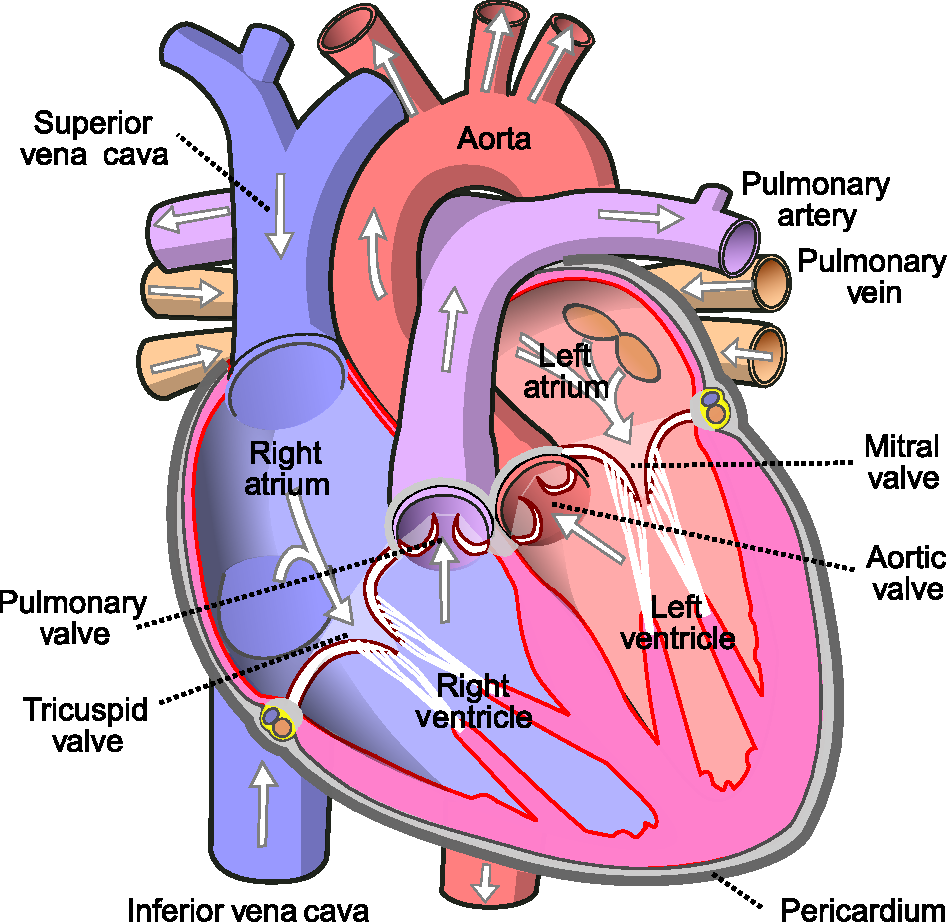
\includegraphics[width=8cm]{figure/Diagram_of_the_human_heart.pdf}
    \caption[Anterior, anatomical view of the structures of a human heart.]{Anterior, anatomical view of a human heart. The primary valves and chambers of the heart are annotated, with arrows indicating the direction of blood flow due to the contractions of the cardiac chambers.
    Image licensed \texttt{CC BY-SA 3.0} from Wikipedia user \href{https://en.wikipedia.org/wiki/User:Wapcaplet}{Wapcaplet}, source: \url{https://en.wikipedia.org/wiki/Heart\#/media/File:Diagram\_of\_the\_human\_heart\_(cropped).svg}.
    }
    \label{fig:heart_anatomy}
\end{figure}

A high level overview of the primary valves and chambers within the heart can be found in Figure~\ref{fig:heart_anatomy}.
The upper chambers of the heart, consisting of the right and left atriums, work in cooperation with the lower chambers of the heart, consisting of the left and right ventricles.
The right ventricle pushes blood into the pulmonary artery which connects to the lungs to return oxygenated blood.
The oxygenated blood returns to the heart through the pulmonary veins and enters into the left atrium.
The left atrium collects ad pumps the oxygenated blood into the left ventricle through the mitral valve.
The left ventricle pumps the oxygenated blood out of the heart to the rest of the body through the aorta.
The deoxygenated blood is collected back into the heart through the superior and inferior vena cava and into the right atrium.
The cycle repeats as the right atrium pumps the blood into the right ventricle through the tricuspid valve, allowing the lungs to once again oxygenate the blood.

\begin{figure}[ht]
    \centering
    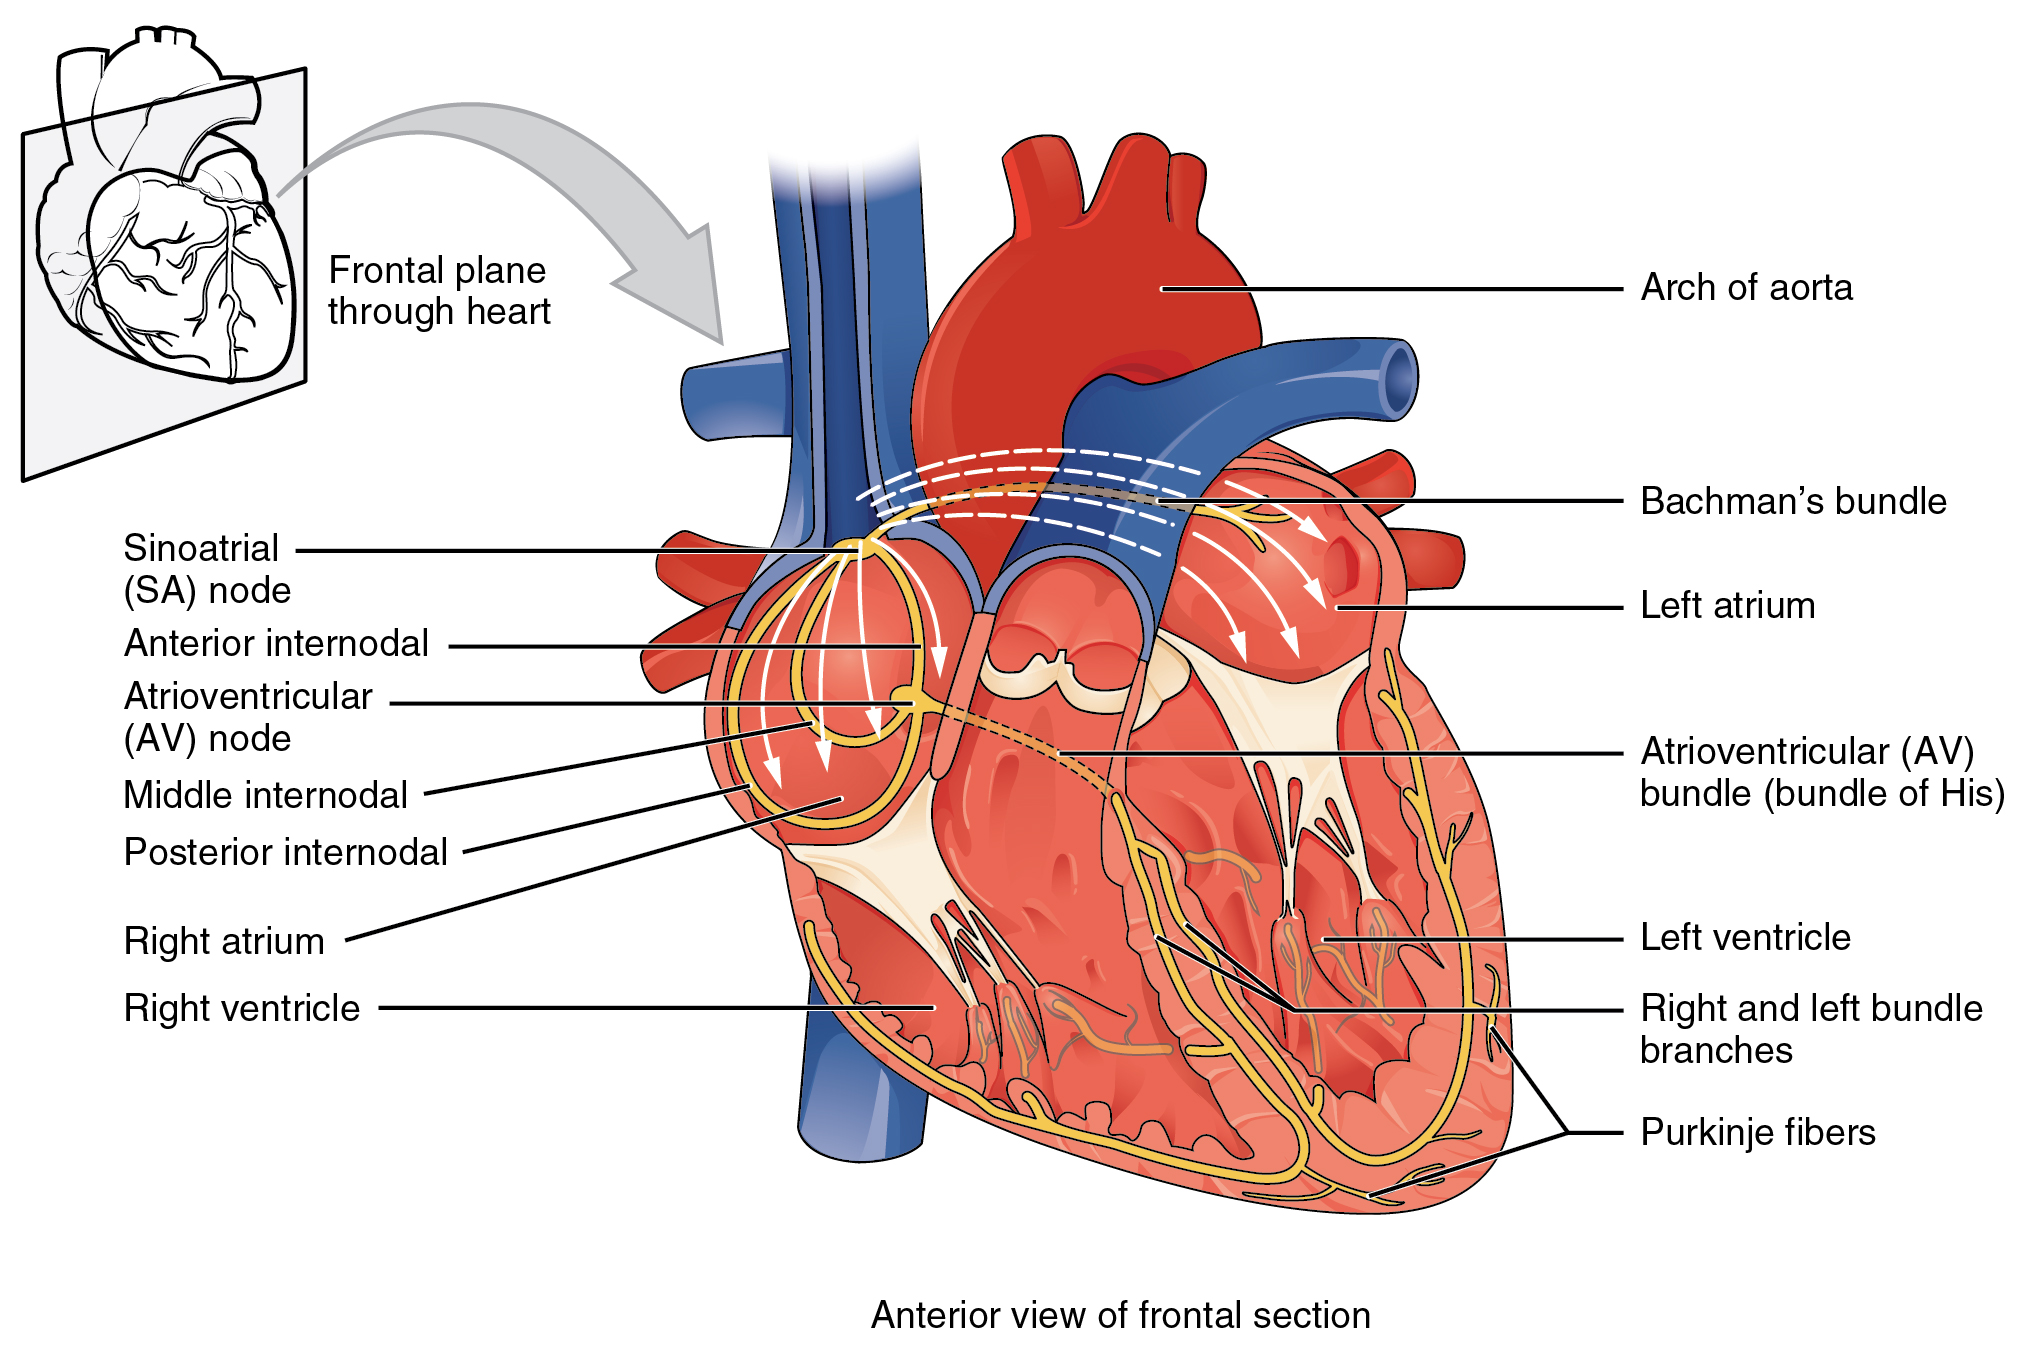
\includegraphics[width=14cm]{figure/conduction-system-of-the-heart.jpeg}
    \caption[Anterior, anatomical view of the conduction system of a human heart.]{Anterior, anatomical view of the conduction system of a human heart. The conducting components of the heart begin with the sinoatrial node and include the internodal pathways, the atrioventricular node, the atrioventricular bundle, the right and left bundle branches, and the Purkinje fibres.
    Image licensed \texttt{CC BY 4.0} from Betts \emph{et al}~\cite{betts-anatomy-and-physiology} on the OpenStax platform, source: \url{https://openstax.org/books/anatomy-and-physiology/pages/19-2-cardiac-muscle-and-electrical-activity\#fig-ch20_02_02}.}
    \label{fig:heart_conduction_system}
\end{figure}

Figure~\ref{fig:heart_conduction_system} shows an overview of the primary structures relevant to the cardiac conduction cycle.
Starting at rest, the sinoatrial node initiates an action potential which travels across the right and left atria.
Once the action potential reaches the atrioventricular node, a ~100ms delay occurs to allow the atria to finish pumping blood before the impluse is sent to the atrioventricular bundle.
Once the delay finishes, the impluse sweeps across the atrioventricular bundle, right and left bundle branches, and to the Purkinje fibers.
Ventricular contraction occurs, then the impulse dissipates at the contractile fibers of the ventricle causing the ventricles to repolarize in preparation for the next heartbeat.

\subsection{Electrocardiogram Tracing}

\begin{figure}[ht]
    \centering
    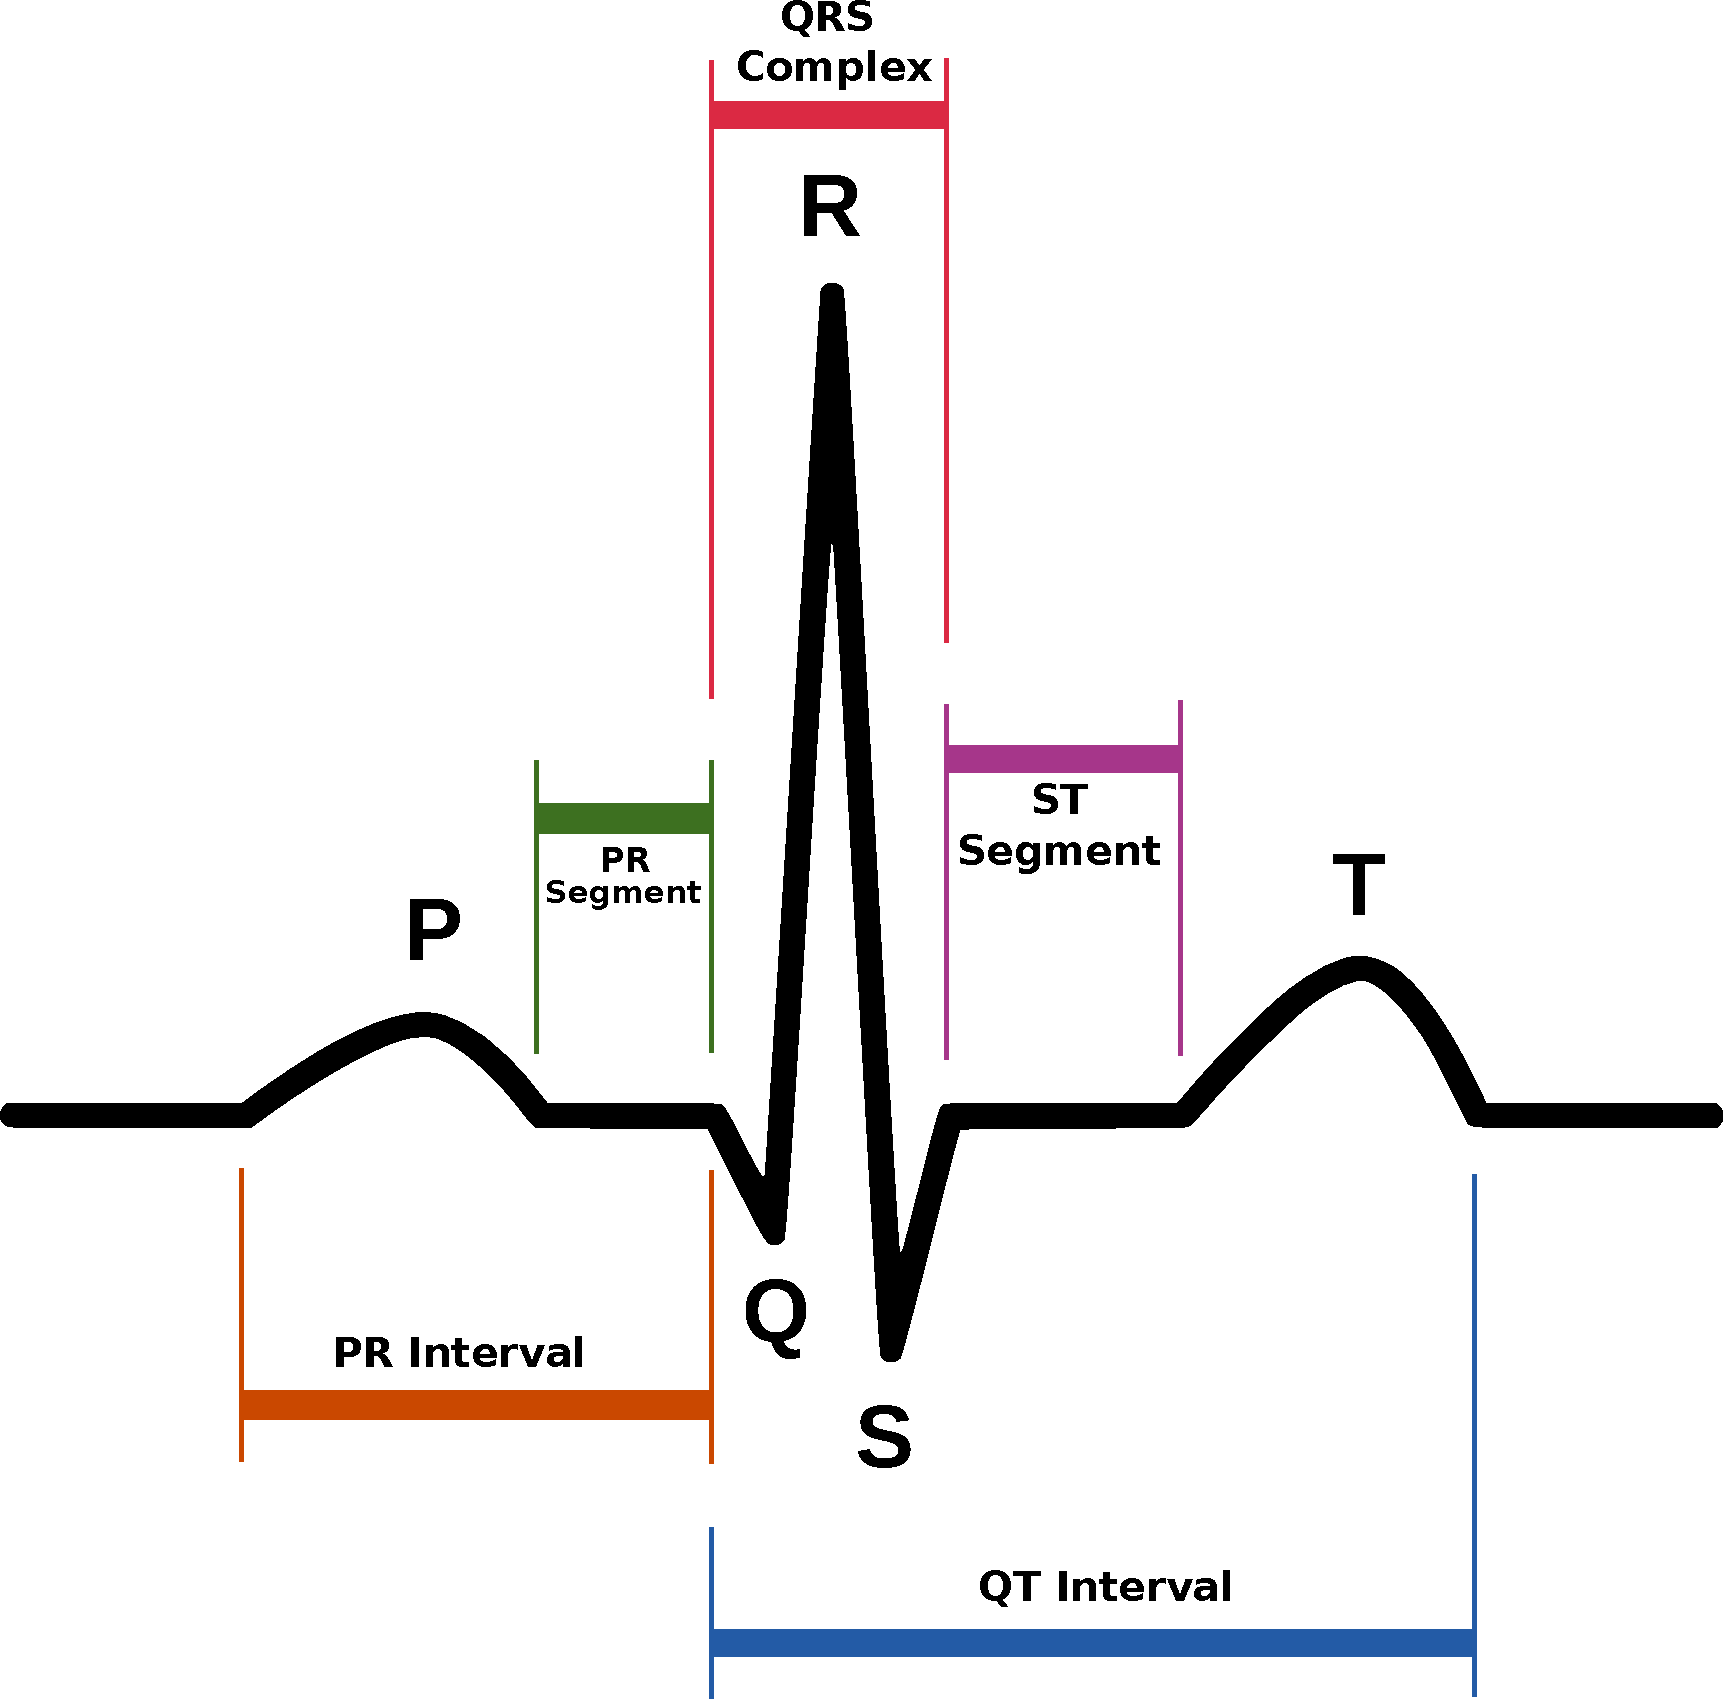
\includegraphics[width=8cm]{figure/PQRST_NormalSinusRhythm.pdf}
    \caption[Normal sinus rhythm \gls{ecg} tracing with PQRST peaks annotated.]{Normal sinus rhythm \gls{ecg} tracing showing the PQRST peaks, the P wave, QRS complex, and T wave along with the PR and QT intervals, plus the PR and ST segments.
    Image belonging to \texttt{public domain} attributed to Anthony Atkielski, source: \url{https://en.wikipedia.org/wiki/Electrocardiography\#/media/File:SinusRhythmLabels.svg}.
    }
    \label{fig:pqrst_nsr}
\end{figure}

Within a typical \gls{ecg}, there are five peaks, labeled PQRST respectively, that define the major components of a heartbeat as shown in Figure~\ref{fig:pqrst_nsr}.
The P wave represents the sinoatrial node initiating an impulse action potential and marks the start of a heartbeat.
The PR segment, which starts after the P wave and ends before the QRS complex, represents the delay between the atrial contraction and the propagation of the signal through the atrioventricular bundle.
The QRS complex is the notable large spike in the \gls{ecg}, which represents the electrical impluse traveling through the atrioventricular bundle and bundle branches to the Purkinje fibers.
The ST segment, starting after the QRS complex and ending before the T wave begins, is the phase of the \gls{ecg} where the actual ventricle contraction occurs.
After the ventricle contraction completes, the impulse dissipates and allows the ventricle muscles to relax and repolarize, manifesting as the \gls{ecg} T wave.
A step by step diagram indicating the different \gls{ecg} tracing components and the corresponding cardiac diagram can be found in Figure~\ref{fig:pqrst_heart_conduction_system}

\begin{figure}[hb]
    \centering
    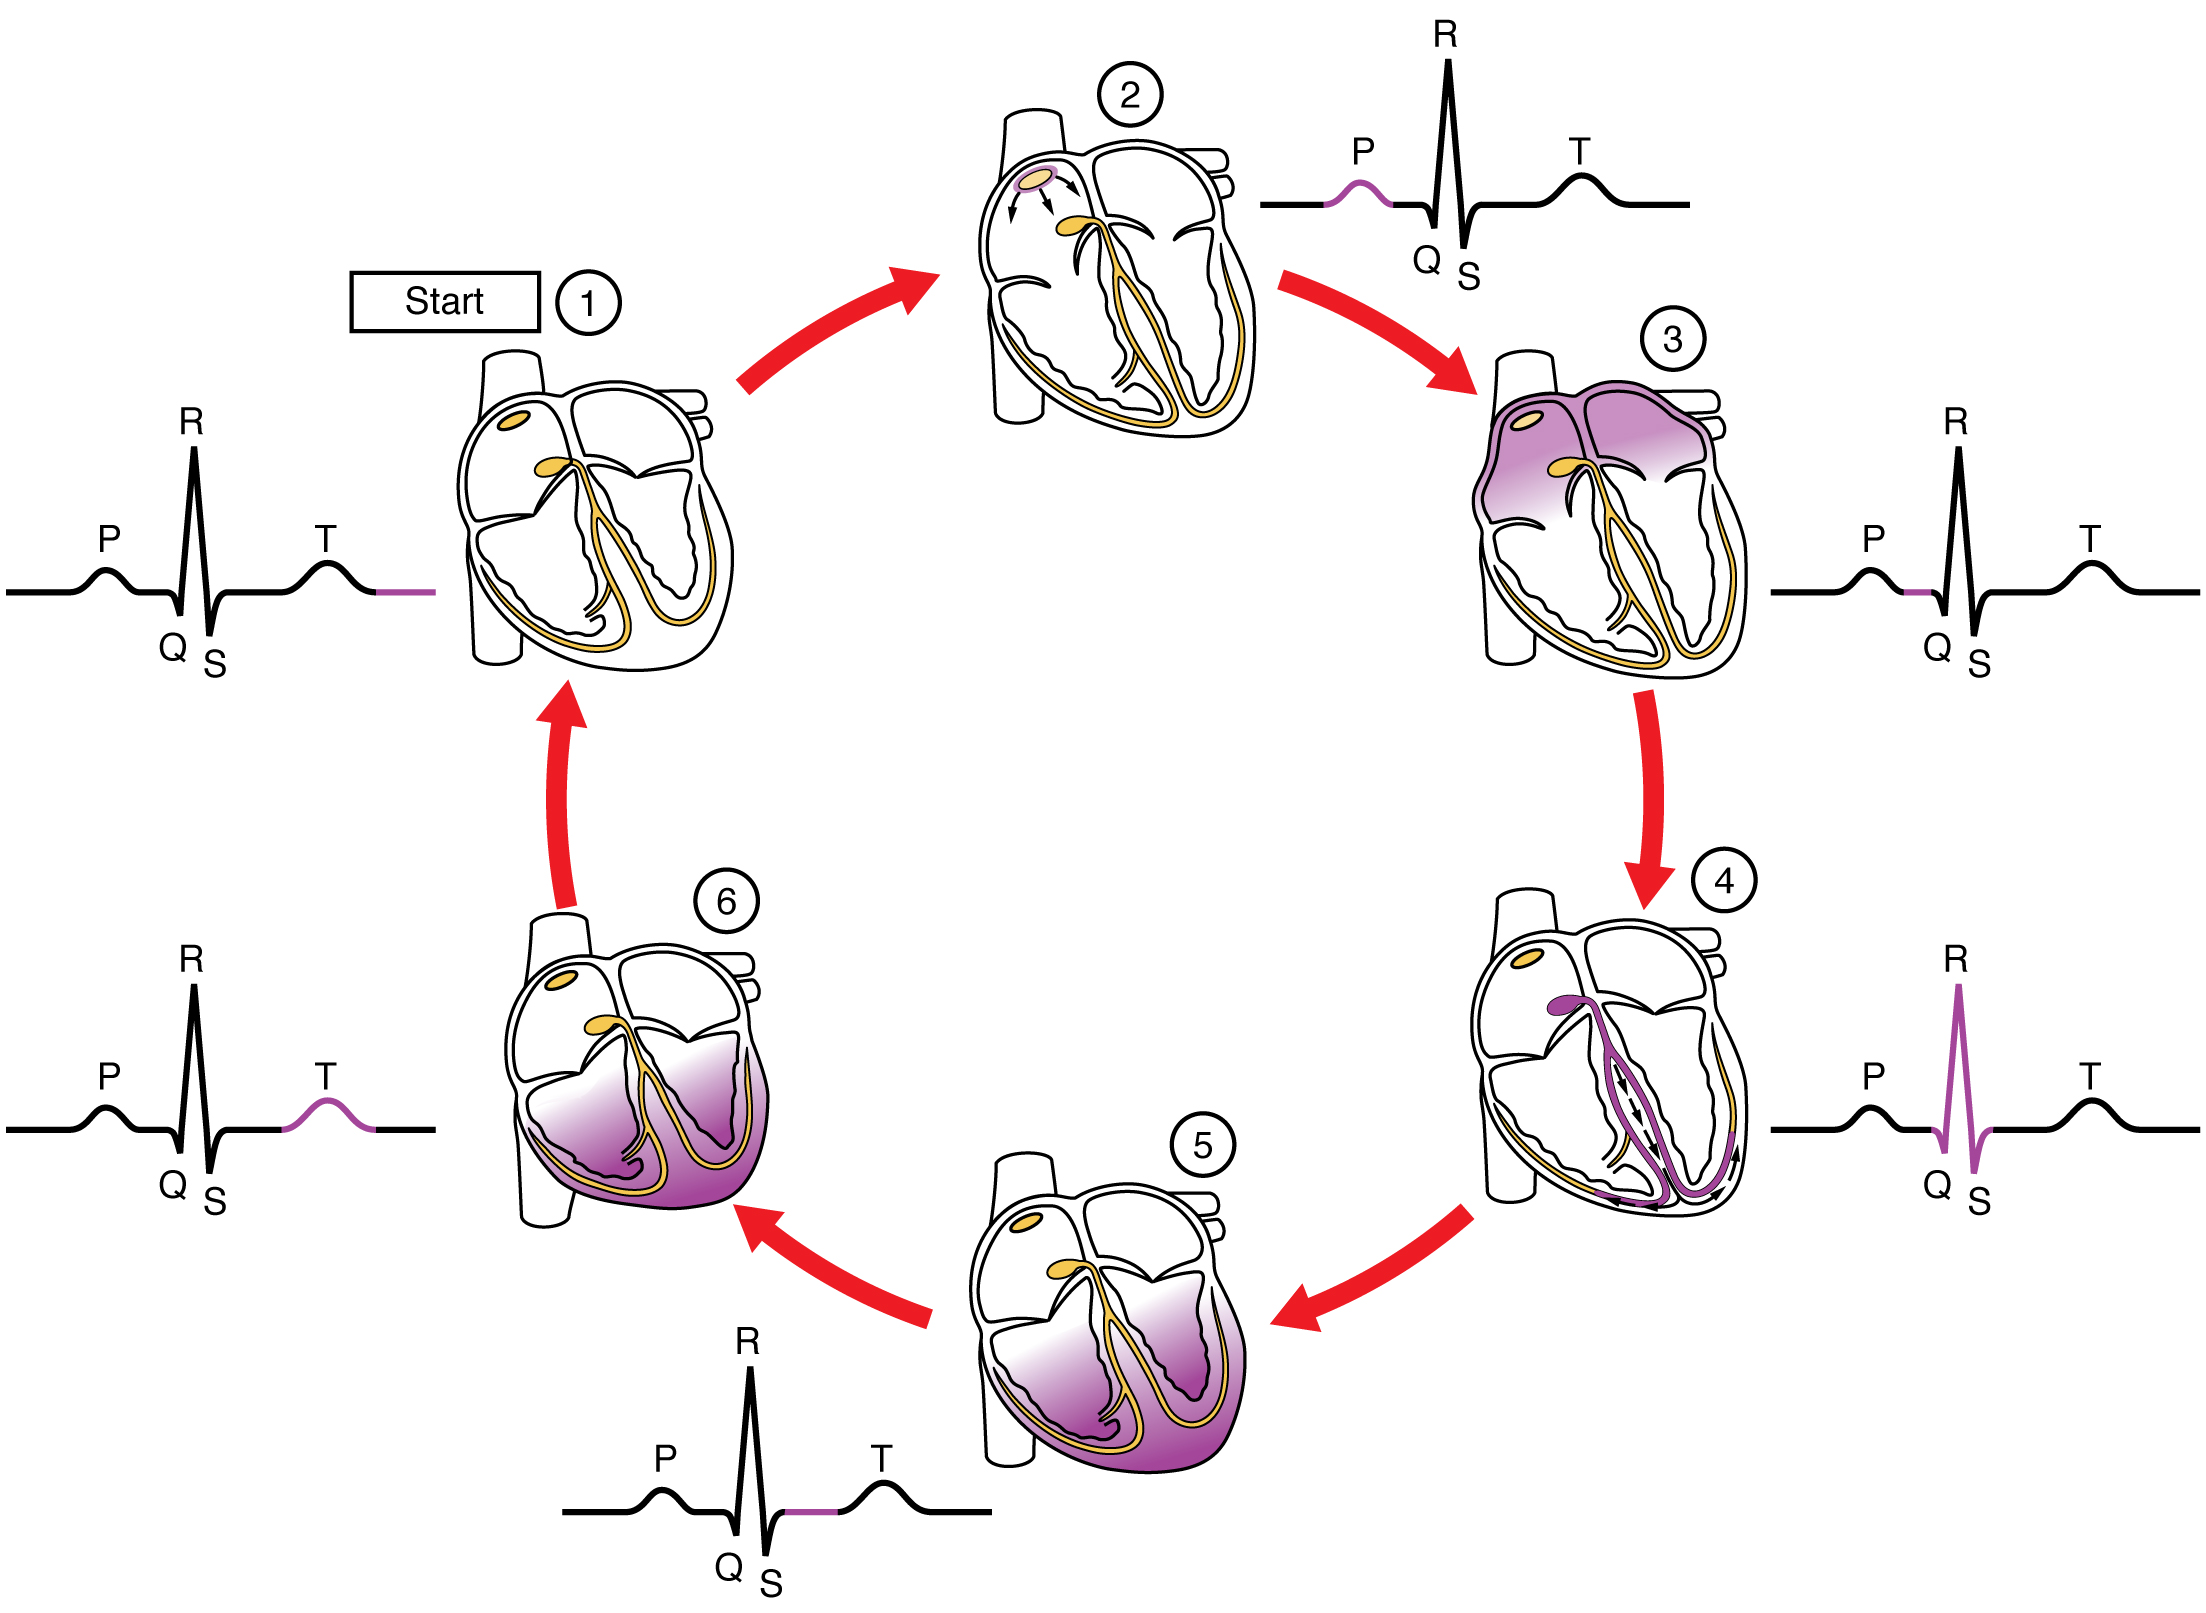
\includegraphics[width=14cm]{figure/pqrst_with_heart_conduction_system.jpeg}
    \caption[Cardiac conduction correlated to ECG tracing waves.]{Cardiac conduction correlated to ECG tracing waves.
    1. The conduction system of the heart is currently at rest, with the ventricles repolarized.
    2. The sinoatrial node begins an action potential which permeates across the atria, causing the \gls{ecg} P wave formation.
    3. A 100ms delay in the impulse occurs which allows the atria to complete pumping blood, showing as the PR segment in the \gls{ecg}.
    4. The impulse proceeds through the atrioventricular bundle and bundle branches to the Purkinje fibers, appearing as the QRS complex in the \gls{ecg}.
    5. The contractile fibers of the ventricles are stimulated by the impulse, causing the ventricles to contract and appears as the ST-segment in the \gls{ecg}.
    6. The impulse dissipates and the ventricular muscles relax, causing the \gls{ecg} T wave formation.
    Image licensed \texttt{CC BY 4.0} from Betts \emph{et al}~\cite{betts-anatomy-and-physiology} on the OpenStax platform, source: \url{https://openstax.org/books/anatomy-and-physiology/pages/19-2-cardiac-muscle-and-electrical-activity\#fig-ch20_02_08}.}
    \label{fig:pqrst_heart_conduction_system}
\end{figure}

\subsection{Electrode Placement and Cardiac Axis}

\begin{figure}[ht]
    \centering
    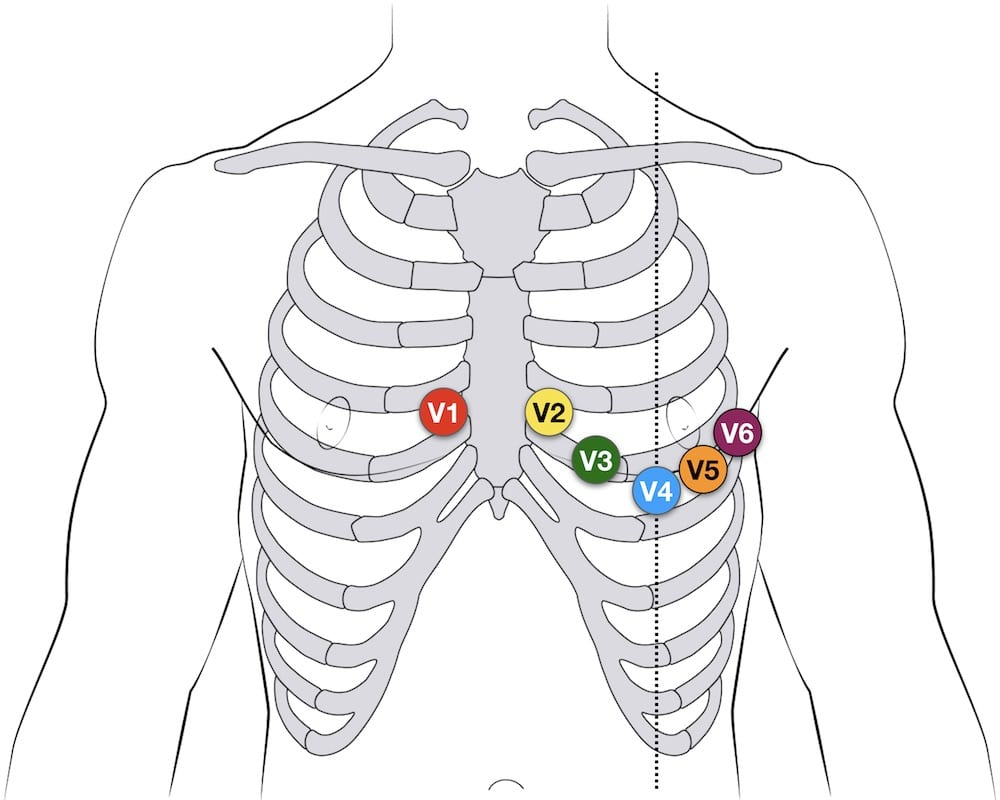
\includegraphics[width=12cm]{figure/12-lead-ECG-lead-placement.jpg}
    \caption[Placement of 12-lead ECG for precordial electrodes V1-V6.]{Placement of 12-lead ECG for precordial electrodes V1-V6. V1 is located in the 4th intercostal space (ICS) on the right margin of the sternum. V2 is placed at the 4th ICS on the left margin of the sternum. V3 is placed midway between V2 and V4. V4 is placed on the 5th ICS mid-clavicular line. V5 is placed on the anterior axillary line at the same level as V4 (5th ICS). V6 is placed on the mid-axillary line at the same level as V4 (5th ICS).
    Image licensed \texttt{CC BY-NC-SA 4.0} from Mike Cadogan~\cite{ecg-lead-positioning} on the Life In The Fast Lane platform, source: \url{https://litfl.com/ecg-lead-positioning/}.}
    \label{fig:12-lead-ecg-placement}
\end{figure}

The 12-lead \gls{ecg} is derived from 10 electrodes placed on the surface of the skin.
The positioning of the leads is critical to ensure that the proper traces are recorded.
See Figure~\ref{fig:12-lead-ecg-placement} for a guide to placing the 6 precordial (front of the heart) leads V1 to V6.
The remaining four leads are extremity or limb electrodes: Right Arm (RA) should be placed anywhere between the right shoulder and right elbow; Right Leg (RL) should be placed below the right torso and above the right ankle; Left Arm (LA) should be placed between the left shoulder and left elbow; and Left Leg (LL) should be placed below the left torso and above the left ankle.

When reading a 12-lead \gls{ecg}, the leads I, II, II, aVR, aVL, and aVF are derived from the limb leads.
Equation~\ref{eq:wilson_central_terminal} shows a common virtual electrode, known as the Wilson's central terminal, defined by averaging three of the limb leads (RA, LA, LL) together.
The unused limb lead RL does not show up in the \gls{ecg} readings and is considered a neutral grounding lead for minimizing artifacts.
See Equation~\ref{eq:lead_I} for lead I, Equation~\ref{eq:lead_II} for lead II, and Equation~\ref{eq:lead_III} for lead III.
The augmented limb leads aVR, aVL, and aVF are derived from the same three electrodes as leads I, II, and III but rely on Wilson's central terminal as their negative pole.
See Equation~\ref{eq:lead_aVR} for lead aVR, Equation~\ref{eq:lead_aVL} for lead aVL, and Equation~\ref{eq:lead_aVF} for lead aVF.
The remaining precordial leads V1 to V6 shown in the ECG are the directly measured signals from the electrodes.

\begin{equation}
    V_W = \dfrac{1}{3}(RA + LA + LL) \label{eq:wilson_central_terminal}
\end{equation}

\begin{equation}
    I = LA - RA \label{eq:lead_I}
\end{equation}

\begin{equation}
    II = LL - RA \label{eq:lead_II}
\end{equation}

\begin{equation}
    III = LL - LA \label{eq:lead_III}
\end{equation}

\begin{equation}
    aVR = \dfrac{3}{2}(RA - V_W) = RA - \dfrac{1}{2}(LA + LL) \label{eq:lead_aVR}
\end{equation}

\begin{equation}
    aVL = \dfrac{3}{2}(LA - V_W) = LA - \dfrac{1}{2}(RA + LL) \label{eq:lead_aVL}
\end{equation}

\begin{equation}
    aVF = \dfrac{3}{2}(LL - V_W) = LL - \dfrac{1}{2}(RA + LA) \label{eq:lead_aVF}
\end{equation}

An \gls{ecg}'s cardiac axis refers to the average direction of the wave of ventricular depolarization measured from the reference point of lead I on a standard 12-lead \gls{ecg}~\cite{meek_introduction_2002}.
One simple estimation of the cardiac axis is done by inspecting the magnitude of the R-peaks on leads I, II, and III.
In a normal \gls{ecg}, leads I, II are positive while lead III may be positive or negative.
There is right axis deviation if lead I is negative and lead III is positive (lead II may be positive or negative).
Left axis deviation exists if lead I is positive while leads II and III are negative.

\begin{figure}
    \centering
    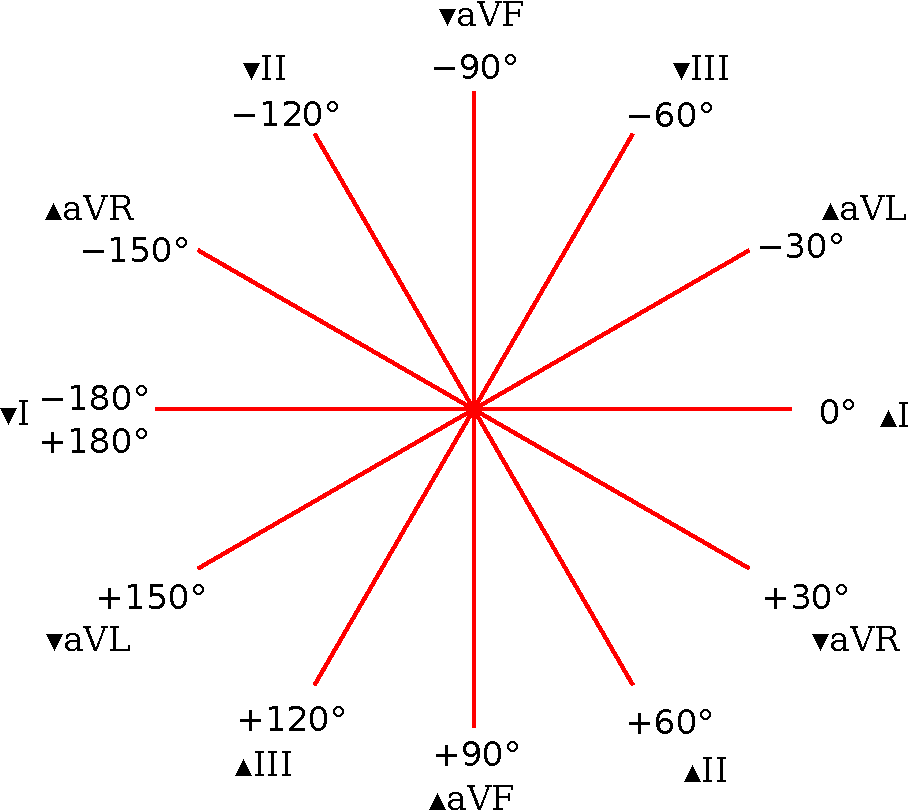
\includegraphics[width=10cm]{figure/Hexaxial_reference_system.pdf}
    \caption{Hexaxial (Cabrera) system for determining cardiac axis. Six frontal planes are viewed in the sequence aVL, I, aVR, II, aVF, and III. Within an ECG record, the lead with the maximum QRS peak amplitude change, positive or negative, is used as the estimate for the cardiac electrical axis.
    Image belonging to \texttt{public domain} from Wikipedia users MoodyGroove and Mysid, source: \url{https://commons.wikimedia.org/w/index.php?curid=2635587}.
    }
    \label{fig:hexaxial_reference}
\end{figure}

Alternatively, the Cabrera system or hexaxial reference system, can be used to logically derive the heart's electrical axis~\cite{lam_classical_2015}.
By viewing the six frontal planes in the sequence aVL, I, aVR, II, aVF, and III, we check the maximal amplitude of the ECG vector (positive or negative) and use it to derive the cardiac electrical axis.
Figure~\ref{fig:hexaxial_reference} shows the hexaxial reference system and the mapping to the six derived limb leads.

\section{PhysioNet/CinC 2020 Challenge Overview}

This chapter summarizes the task of multi-label, multi-class classification of \gls{ecg}s as proposed by Perez Alday \emph{et al.}~\cite{physionet_challenge_2020} in the \emph{PhysioNet/CinC 2020 Challenge}.

\subsection{Public Dataset}
The challenge provided a public collection of 43,101 labelled \gls{ecg} records for training.
These public records were sourced from multiple locations, including:

\begin{enumerate}
    \item The China Physiological Signal Challenge (\textbf{CPSC}) 2018~\cite{liu_open_2018} corpus of data, containing 10,330 recordings.
    \item The St. Petersburg Institute of Cardiological Technics (\textbf{INCART}) database of 12-lead arrhythmias~\cite{tihonenko2008st}, containing 74 recordings.
    \item The Physikalisch Technische Bundesanstalt (PTB) contributed datasets \textbf{PTB} Diagnostic \gls{ecg} Database~\cite{NutzungderEKGSignaldatenbankCARDIODATderPTBberdasInternet} and the more recent \textbf{PTB-XL} database~\cite{wagner_ptb-xl_2020}, containing a combined total of 22,353 records
    \item The Georgia 12-lead \gls{ecg} Challenge (\textbf{G12EC}) database, containing 10,344 records.
\end{enumerate}

A separate hold-out set of \gls{ecg} records is sourced from an undisclosed organization containing patients geographically distinct from the publicly available data.
This hold-out set of data is used for the official challenge test phase only and is not available to researchers.
In my analysis, I do not make any distinction between the different \gls{ecg} source locations and combine all of the records into a single repository.
Two \gls{ecg} records (\texttt{Training\_2/Q0400}, \texttt{Training\_2/Q2961} from the CPSC2018 tranche of signals) containing no activity on any leads are excluded from analysis.

\begin{figure}[ht]
    \centering
    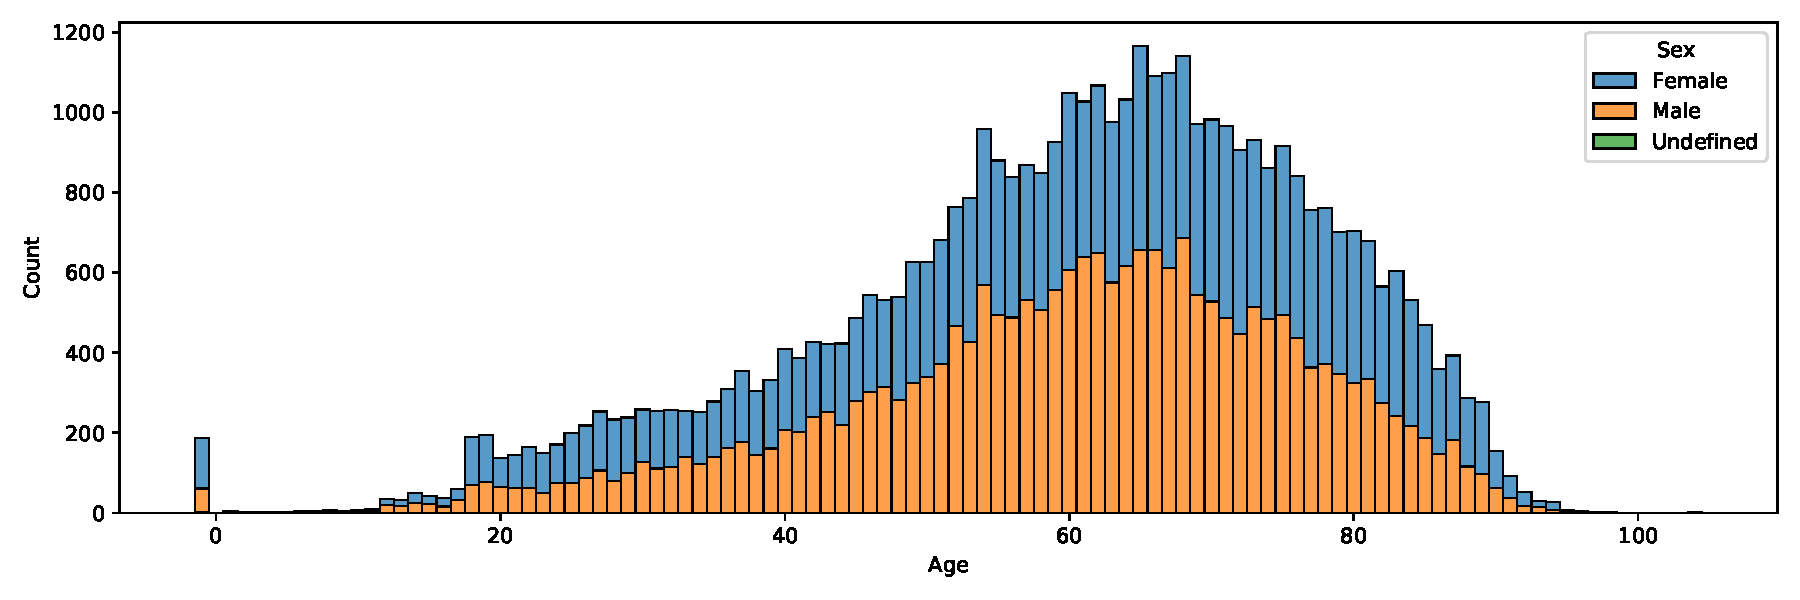
\includegraphics[width=14cm]{figure/age_sex_hist.pdf}
    \caption[Age and sex distribution of the PhysioNet/CinC 2020 public electrocardiogram dataset.]{Age and sex distribution of the PhysioNet/CinC 2020 public electrocardiogram dataset.
    Records with age $<0$ indicate that age is not provided for the given record. The only record that is missing the biological sex metadata is also missing the age metadata.}
    \label{fig:age_sex_hist}
\end{figure}

Each \gls{ecg} record also contains additional metadata in the form of the patient age and biological sex.
There are 187 records that contain an undefined age.
Of the remaining records, the mean patient age is 60.3.
The \gls{ecg} records contained primarily male and female sex, with 46.9\% of the patients in the dataset as female, 53.1\% of the patients as male, and one record that did not have the sex metadata specified.
A histogram showcasing the distribution of the age and sex in our dataset can be found in Figure~\ref{fig:age_sex_hist}.

\subsection{Diagnosed Labels}

\begin{table}[t]
    \caption{\label{tab:labels_snomed_ct} Evaluated SNOMED CT codes with definition, count and percentage in dataset.}
    \vspace{2 mm}
    \centerline{\begin{tabular}{@{}ll@{}l@{}r@{}}
    SNOMED & Abbr. & Diagnosis & Count (\%) \\ \hline
    270492004 & IAVB & 1st degree av block & 2394 (5.6\%) \\
    164889003 & AF & atrial fibrillation & 3475 (8.0\%) \\
    164890007 & AFL & atrial flutter & 314 (0.7\%) \\
    426627000 & Brady & bradycardia & 288 (0.7\%) \\
    713427006 & CRBBB & complete right bundle branch block & 683 (1.6\%) \\
    713426002 & IRBBB & incomplete right bundle branch block & 1611 (3.7\%) \\
    445118002 & LAnFB & left anterior fascicular block & 1806 (4.2\%) \\
    39732003 & LAD & left axis deviation & 6086 (14.1\%)  \\
    164909002 & LBBB & left bundle branch block & 1041 (2.4\%) \\
    251146004 & LQRSV & low QRS voltages & 556 (1.3\%) \\
    698252002 & {{NSIVCB }} & nonspecific intraventricular conduction & 997 (2.3\%) \\
    10370003 & PR & pacing rhythm & 299 (0.7\%) \\
    284470004 & PAC & premature atrial contraction & 1729 (4.0\%) \\
    427172004 & PVC & premature ventricular contractions & 188 (0.4\%) \\
    164947007 & LPR & prolonged PR interval & 340 (0.7\%) \\
    111975006 & LQT & prolonged QT interval & 1513 (3.5\%) \\
    164917005 & QAb & Q wave abnormal & 1013 (2.4\%) \\
    47665007 & RAD & right axis deviation & 427 (1.0\%) \\
    59118001 & RBBB & right bundle branch block & 2402 (5.6\%) \\
    427393009 & SA & sinus arrhythmia & 1240 (2.9\%) \\
    426177001 & SB & sinus bradycardia & 2359 (5.5\%) \\
    426783006 & SNR & sinus rhythm & 20846 (48.4\%)  \\
    427084000 & STach & sinus tachycardia & 2402 (5.6\%) \\
    63593006 & SVPB & supraventricular premature beats & 215 (0.5\%) \\
    164934002 & TAb & T wave abnormal & 4673 (10.8\%)  \\
    59931005 & TInv & T wave inversion & 1112 (2.6\%) \\
    17338001 & VPB & ventricular premature beats & 365 (0.8\%) \\ \hline
    \end{tabular}}
\end{table}

Each record in our available dataset is labelled with at least one numerical \gls{snomed} clinical term (CT).
For the purpose of the challenge, a subset of 27 codes/labels have been selected for classification.
All other codes are ignored in this study.
Please refer to Table~\ref{tab:labels_snomed_ct} for the labels, abbreviations, counts, and proportion within the dataset.

\begin{description}
    \begin{figure}[ht]
        \centering
        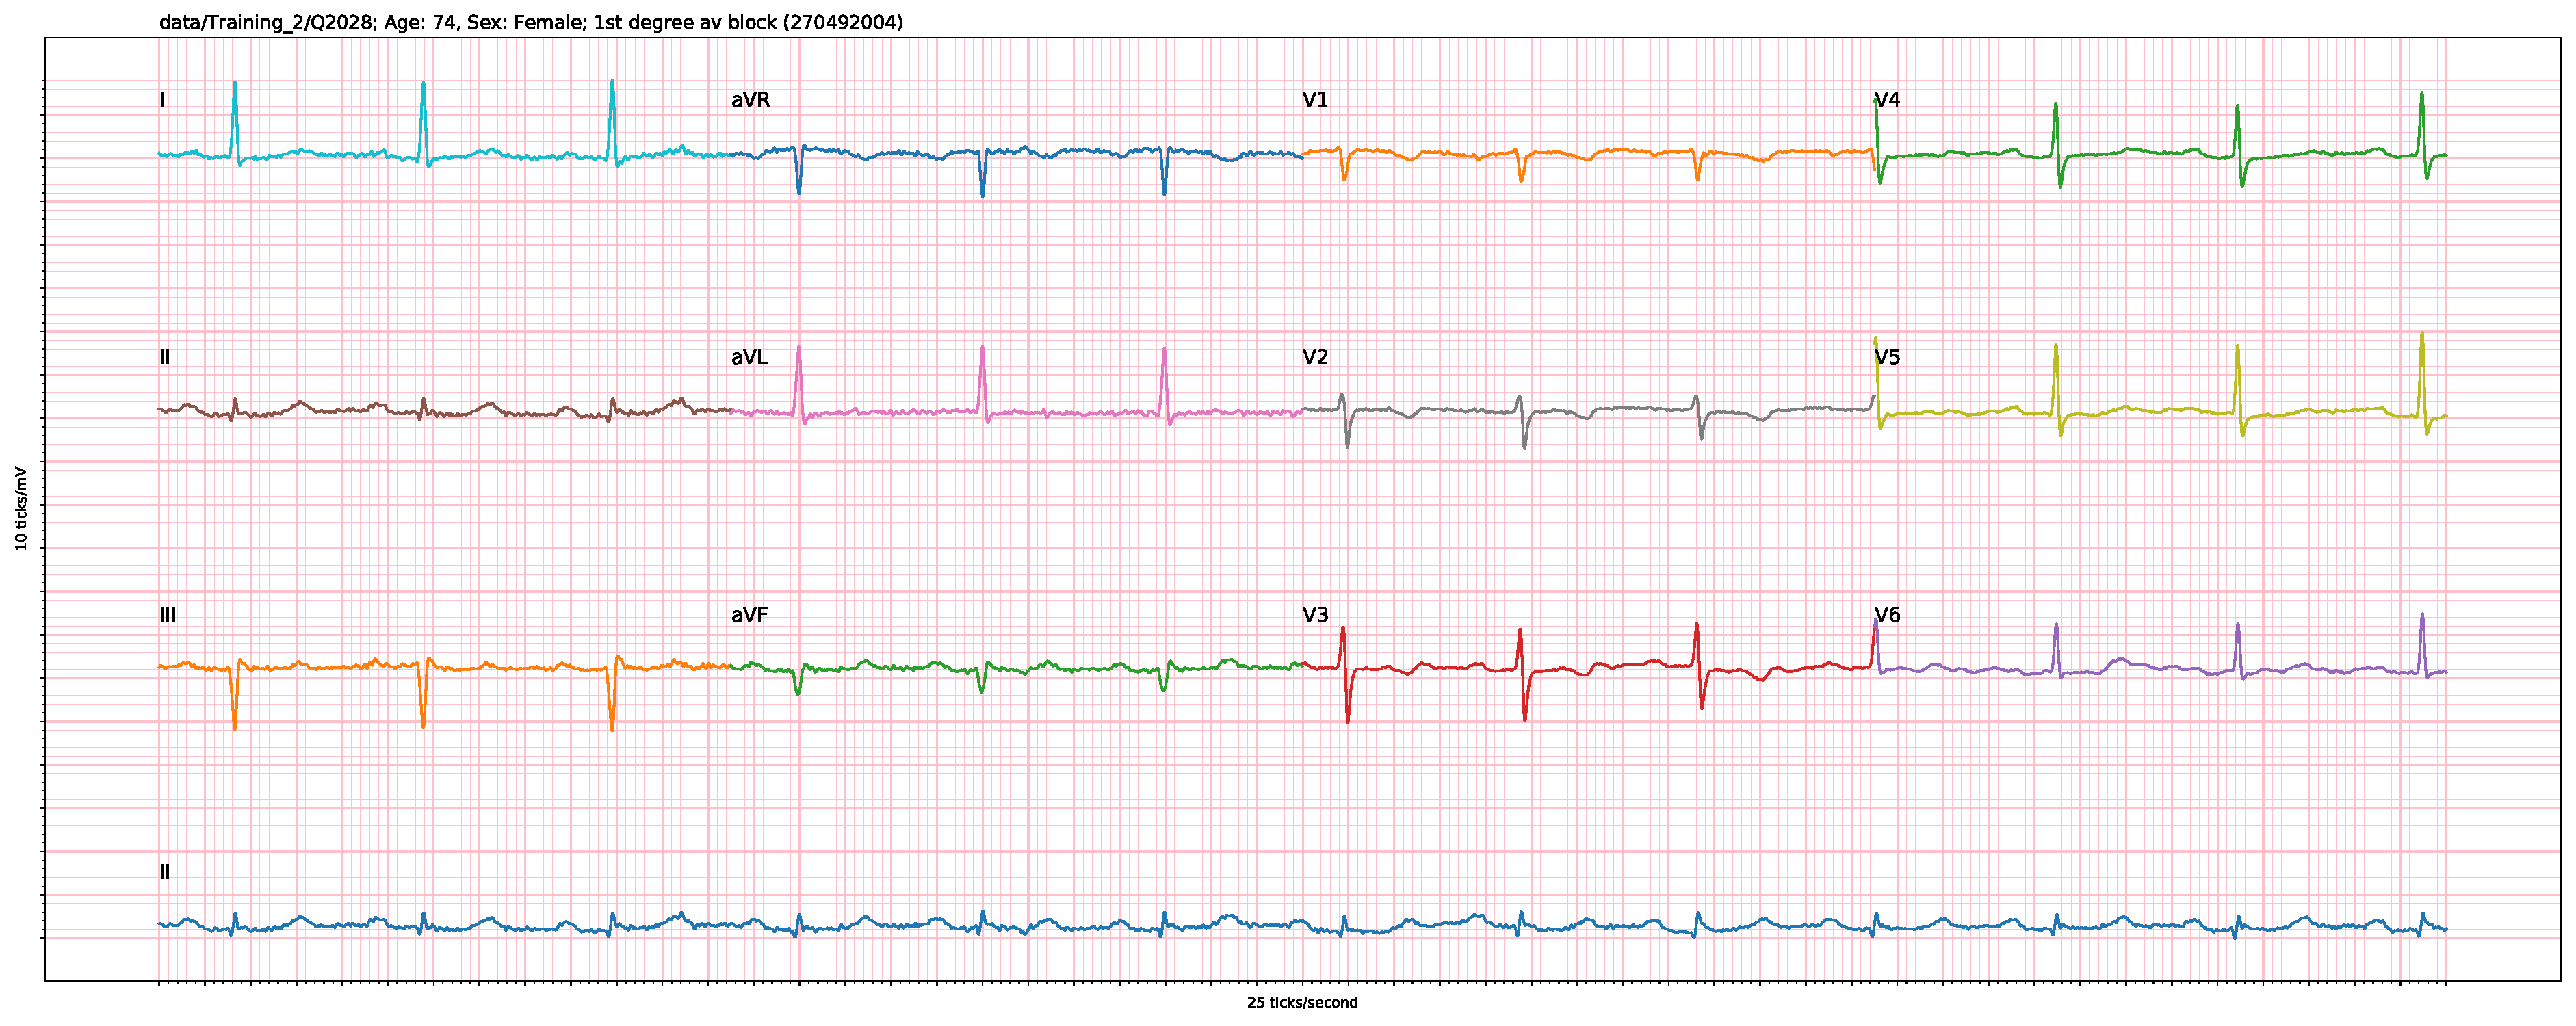
\includegraphics[width=14cm]{figure/IAVB/full_0_1951.pdf}
        \caption{Instance of \gls{ecg} record with 1st degree av block. Long PR interval greater than 200ms is observed.}
        \label{fig:full_IAVB}
    \end{figure}
    \item[\gls{iavb}] This is when there is an abnormally long delay between the electrical impulse from the atria, through the ventricular node, to the ventricles. On the \gls{ecg}, this is detected by the presence of a PR interval longer than 200ms~\cite{carroz_pseudo-pacemaker_2010} or by the existence of a notched (bimodal) P-wave in leads I, II, III, and aVF~\cite{bayes_de_luna_diagnosis_2017}. See Figure~\ref{fig:full_IAVB} for an example of an \gls{ecg} record containing this ailment.
    \begin{figure}[ht]
        \centering
        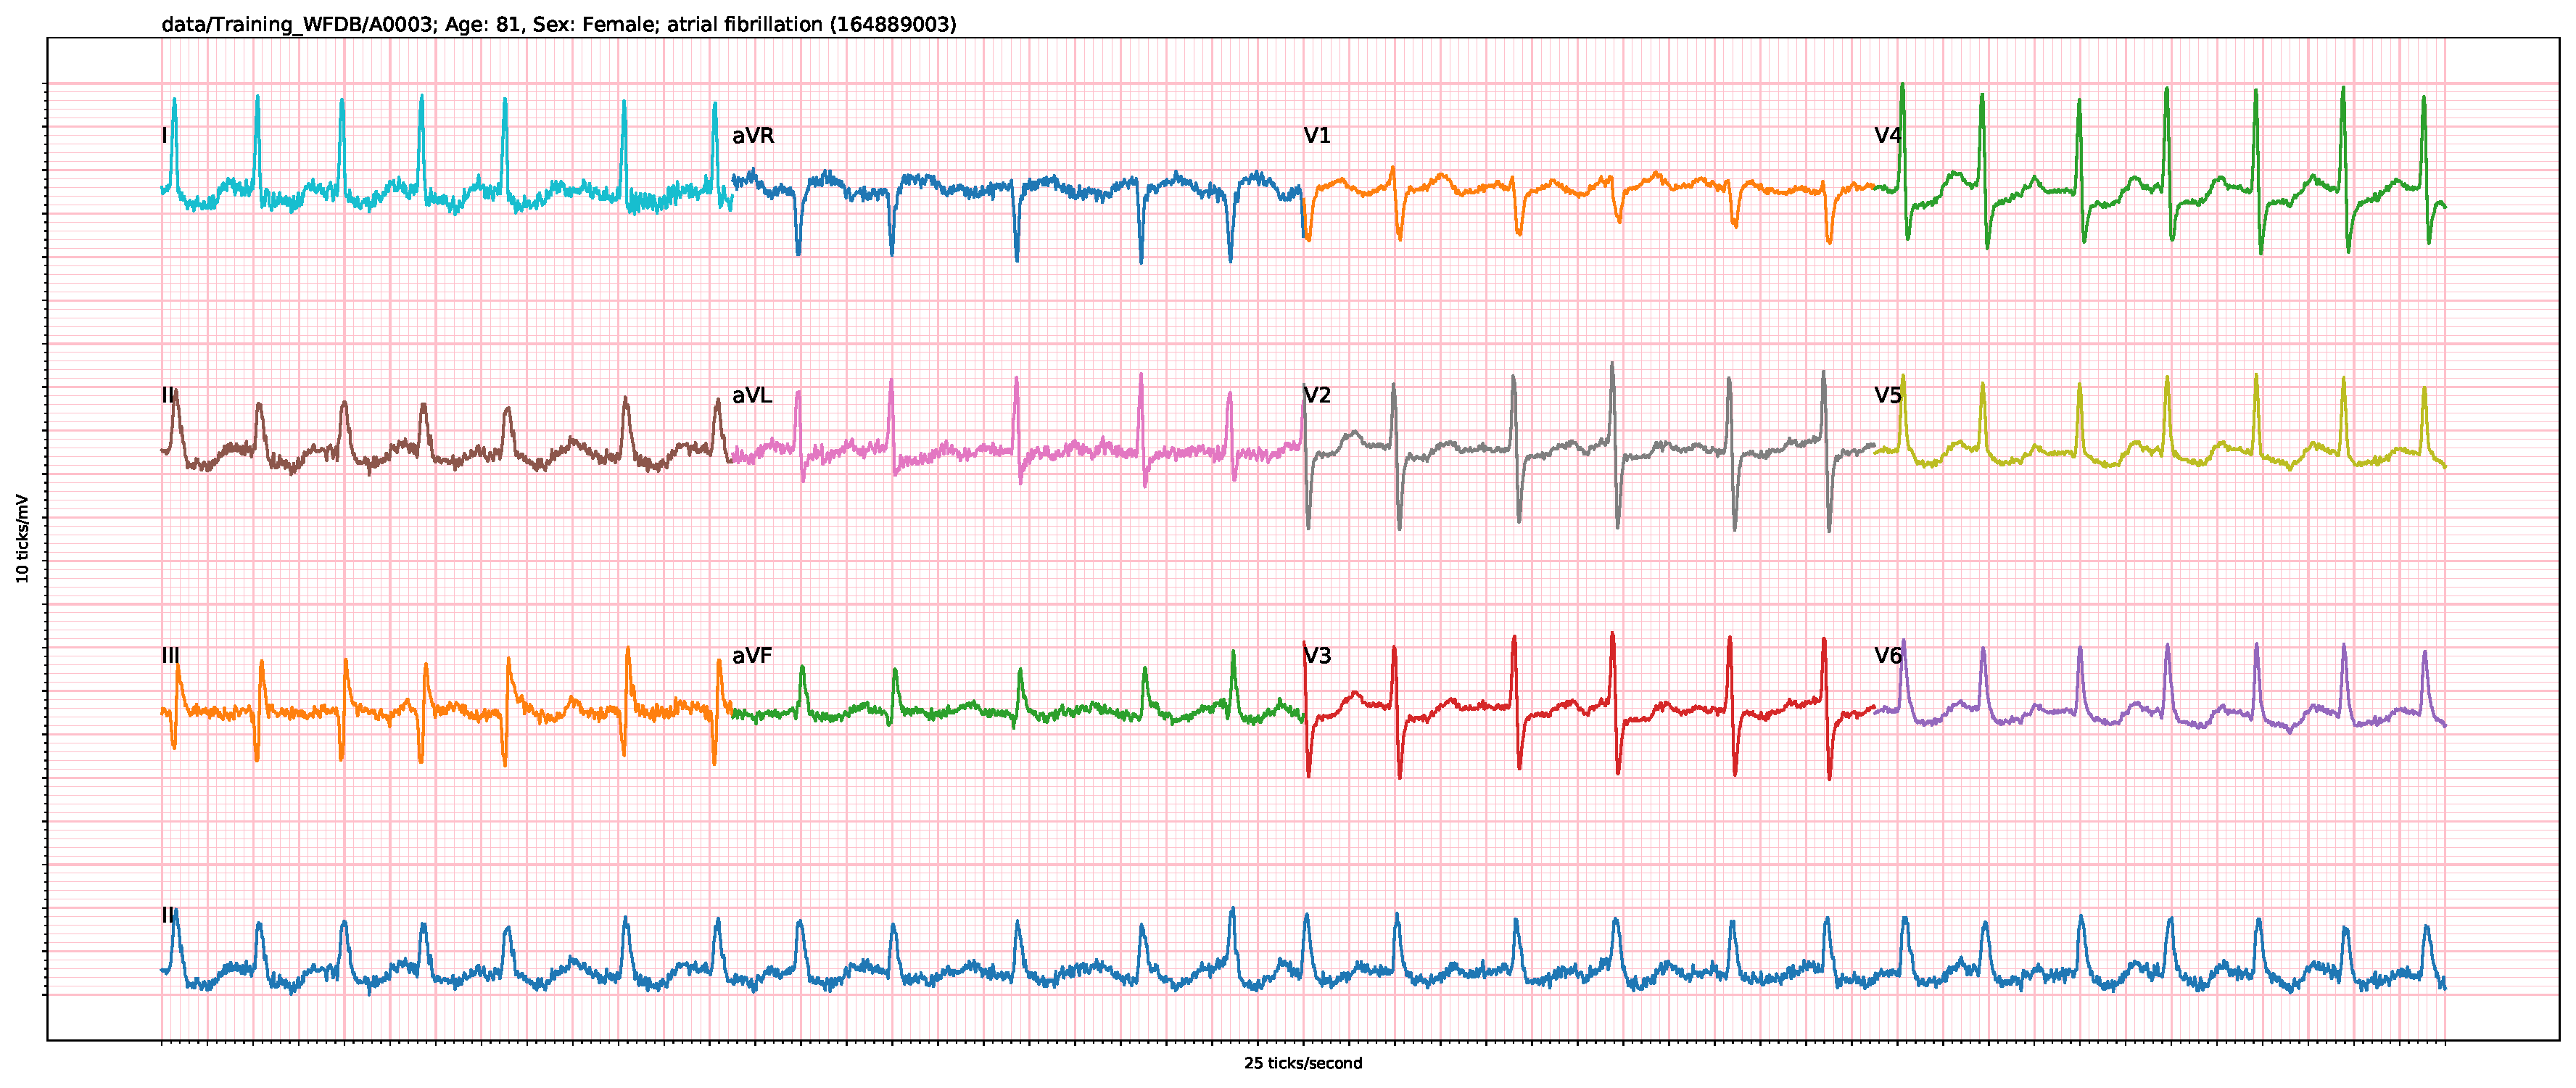
\includegraphics[width=14cm]{figure/AF/full_0_3453.pdf}
        \caption{Instance of 12-lead \gls{ecg} with atrial fibrillation. Irregular, fibrillatory p-waves found in all leads.}
        \label{fig:full_AF}
    \end{figure}
    \item[\gls{af}] The manifestation of \gls{af} may take on multiple forms, ranging from the absence of P waves, irregular heartbeat rhythm, or fibrillatory (rapid, fluttering) P-waves~\cite{podrid2001cardiac,afib-ecg}. Figure~\ref{fig:full_AF} shows an \gls{ecg} instance with this disorder.
    \begin{figure}[ht]
        \centering
        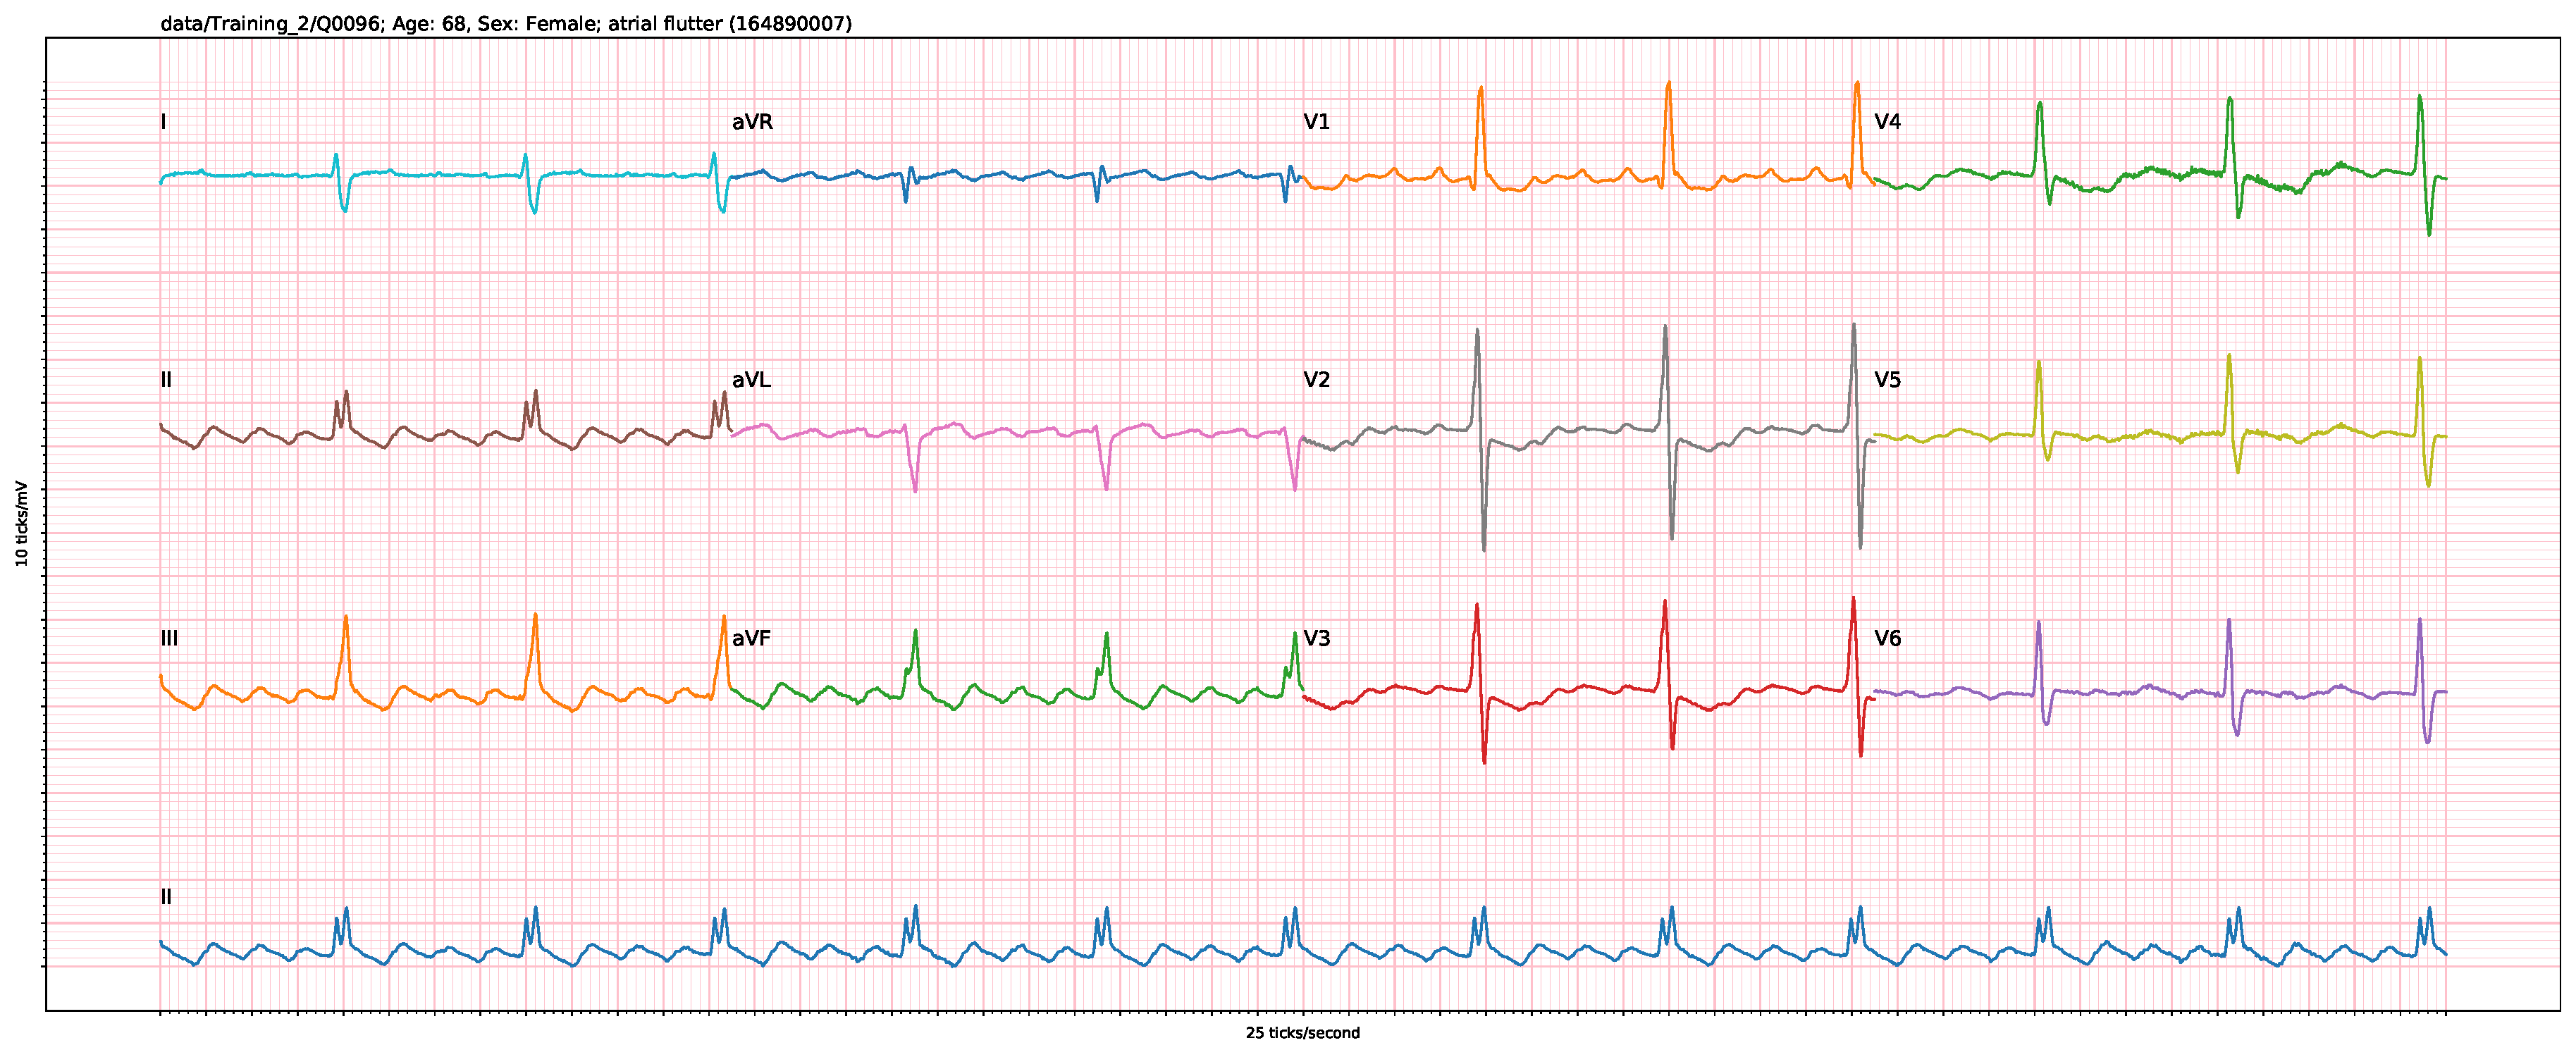
\includegraphics[width=14cm]{figure/AFL/full_0_93.pdf}
        \caption{Instance of 12-lead \gls{ecg} with atrial flutter. Rapid P waves exist.}
        \label{fig:full_AFL}
    \end{figure}
    \item[\gls{afl}] This disorder is indicated by the presence of atrial rhythms at a constant rate $\geq 100$ beats per minute~\cite{saoudi_classification_2001}. Figure~\ref{fig:full_AFL} shows an \gls{ecg} instance with rapid and well-formed P waves.
    \begin{figure}
        \centering
        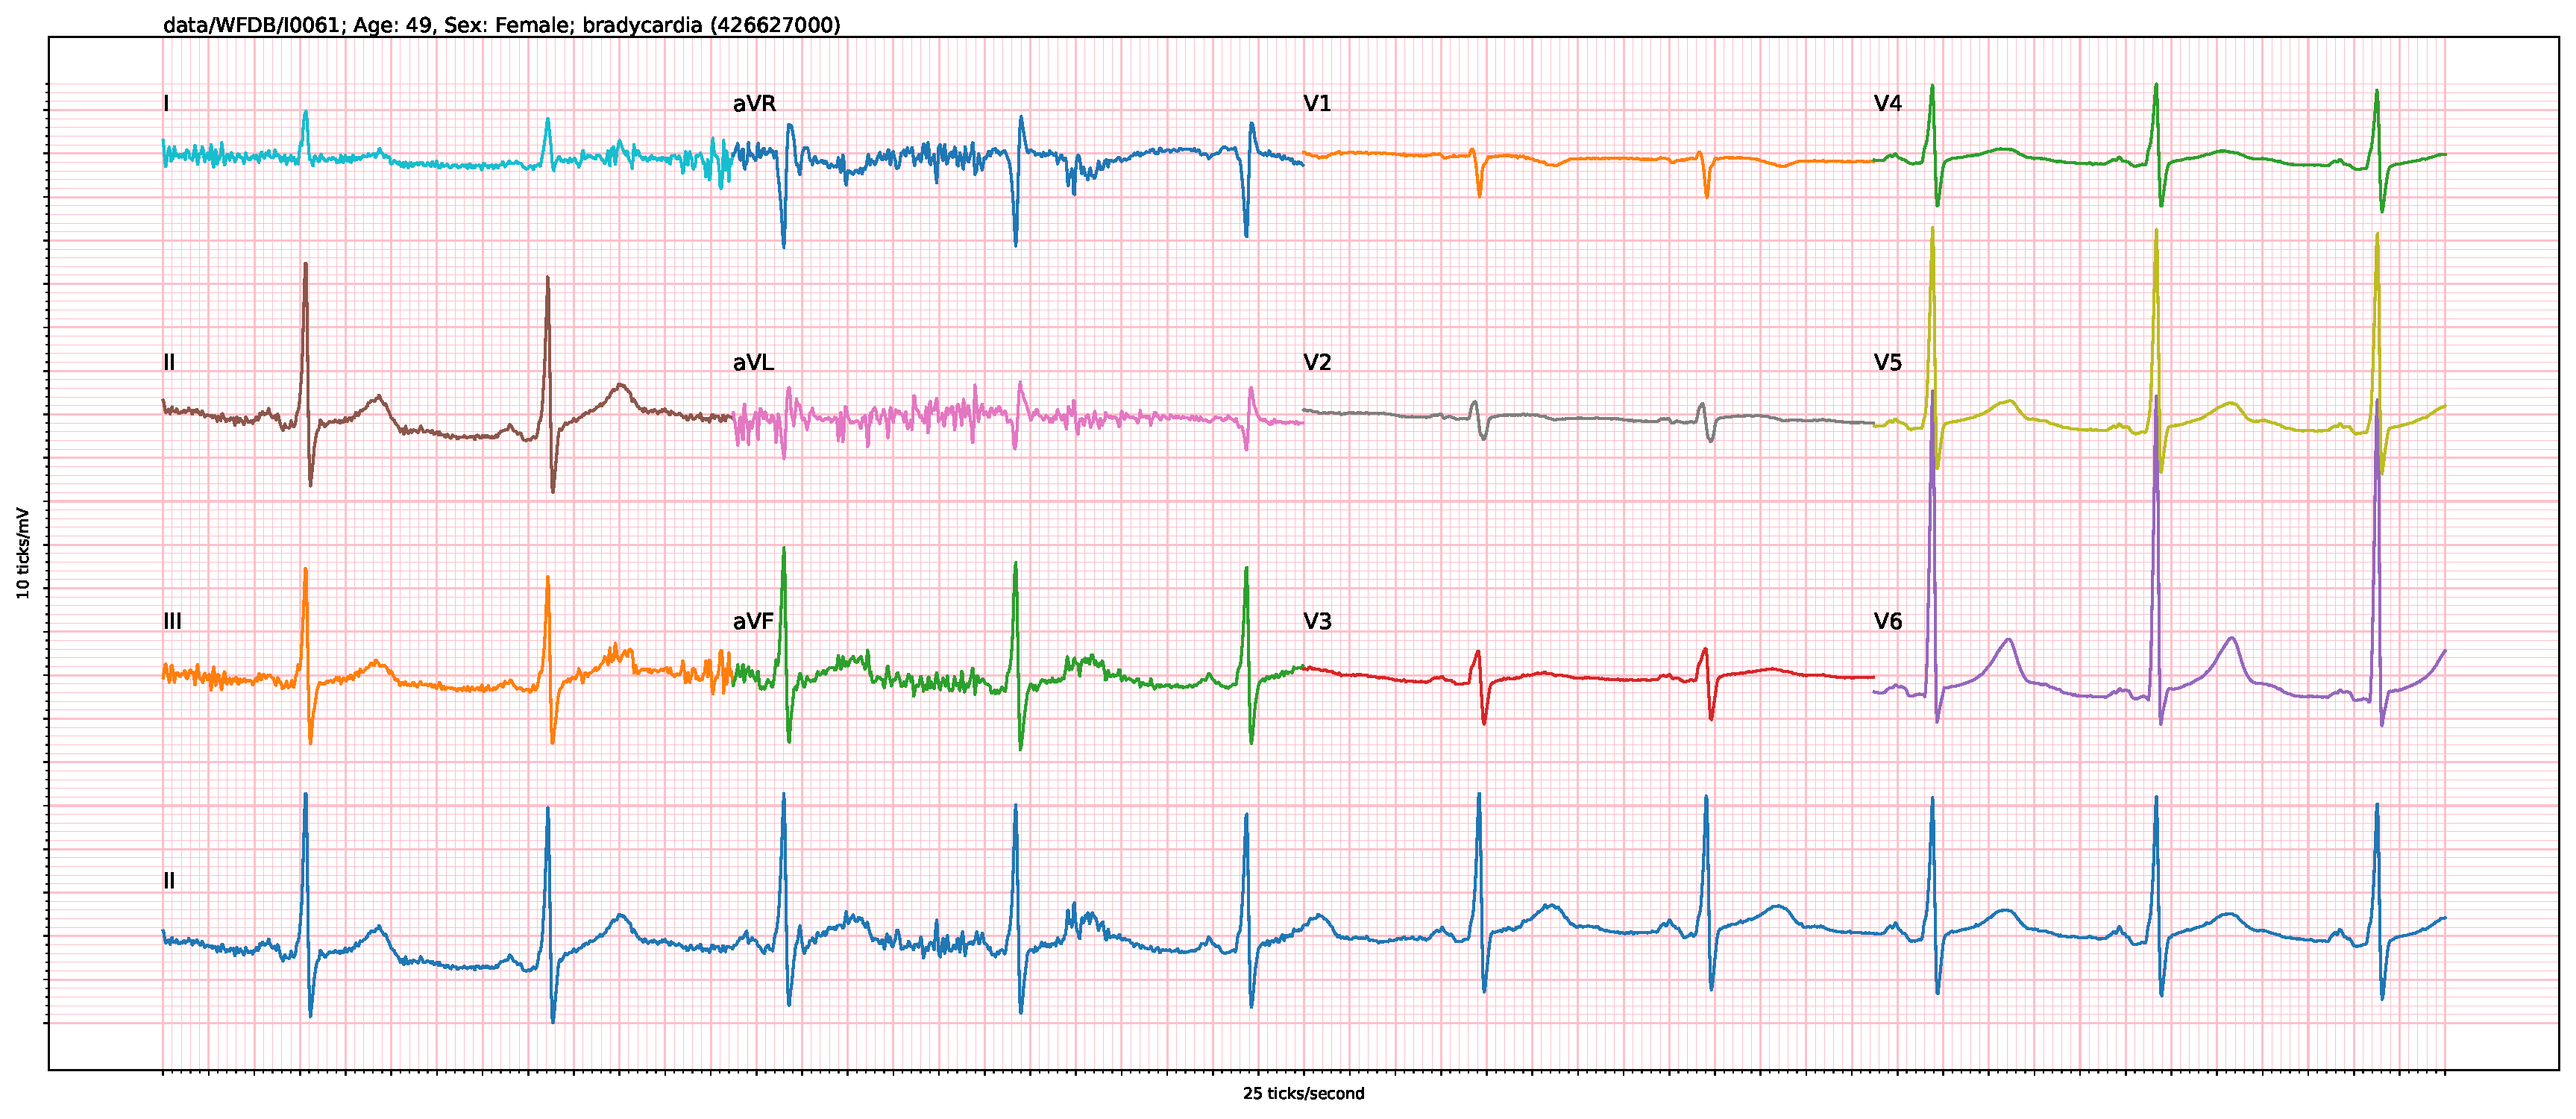
\includegraphics[width=14cm]{figure/Brady/full_0_42568.pdf}
        \caption{Instance of 12-lead \gls{ecg} with bradycardia. Patient has a mean resting heart rate of 57 beats per minute.}
        \label{fig:full_Brady}
    \end{figure} 
    \item[\gls{brady}] A patient has bradycardia if their sinus rhythm is below the normal range of for the age of the patient. For adults, this is a resting heart rate below 60 beats per minute. An example of a patient with bradycardia is shown in Figure~\ref{fig:full_Brady}.
    \begin{figure}
        \centering
        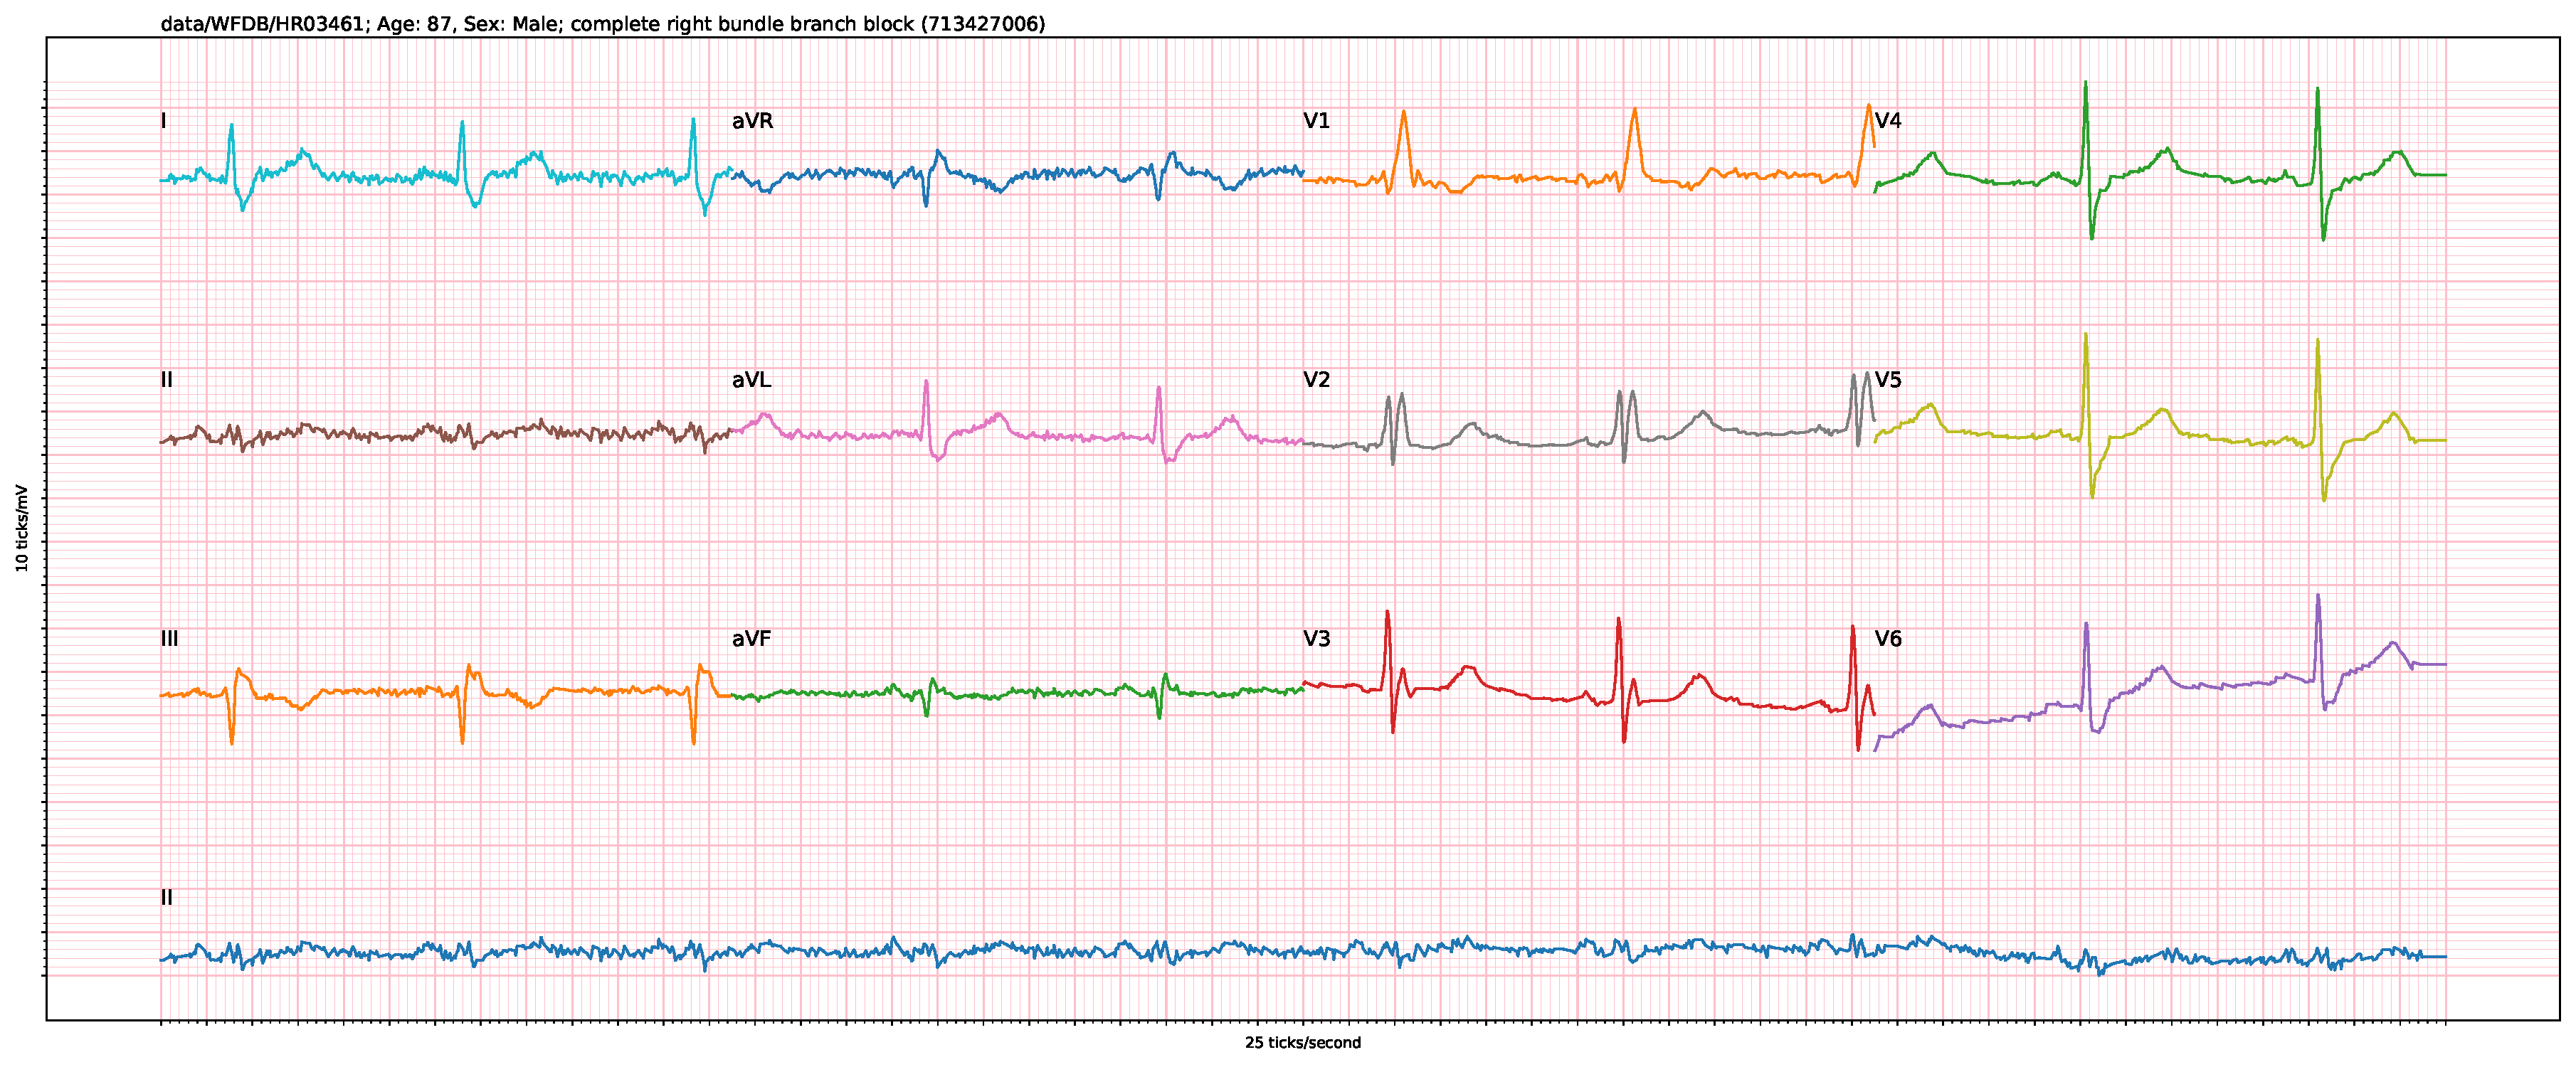
\includegraphics[width=14cm]{figure/CRBBB/full_2_24132.pdf}
        \caption{Instance of 12-lead \gls{ecg} with complete right bundle branch block. QRS complex exceeds 120 ms (4 boxes) and contains an anterior skew on the right end of the QRS complex.}
        \label{fig:full_CRBBB}
    \end{figure} 
    \item[\gls{crbbb}] A complete right bundle branch block is when the QRS duration exceeds 120 ms and the terminal halves of the QRS are skewed rightward and anteriorly, indicating that the right ventricle is being depolarized after the left ventricle~\cite{ecg-utah-lesson}. An example \gls{ecg} record is shown in Figure~\ref{fig:full_CRBBB}.
    \begin{figure}
        \centering
        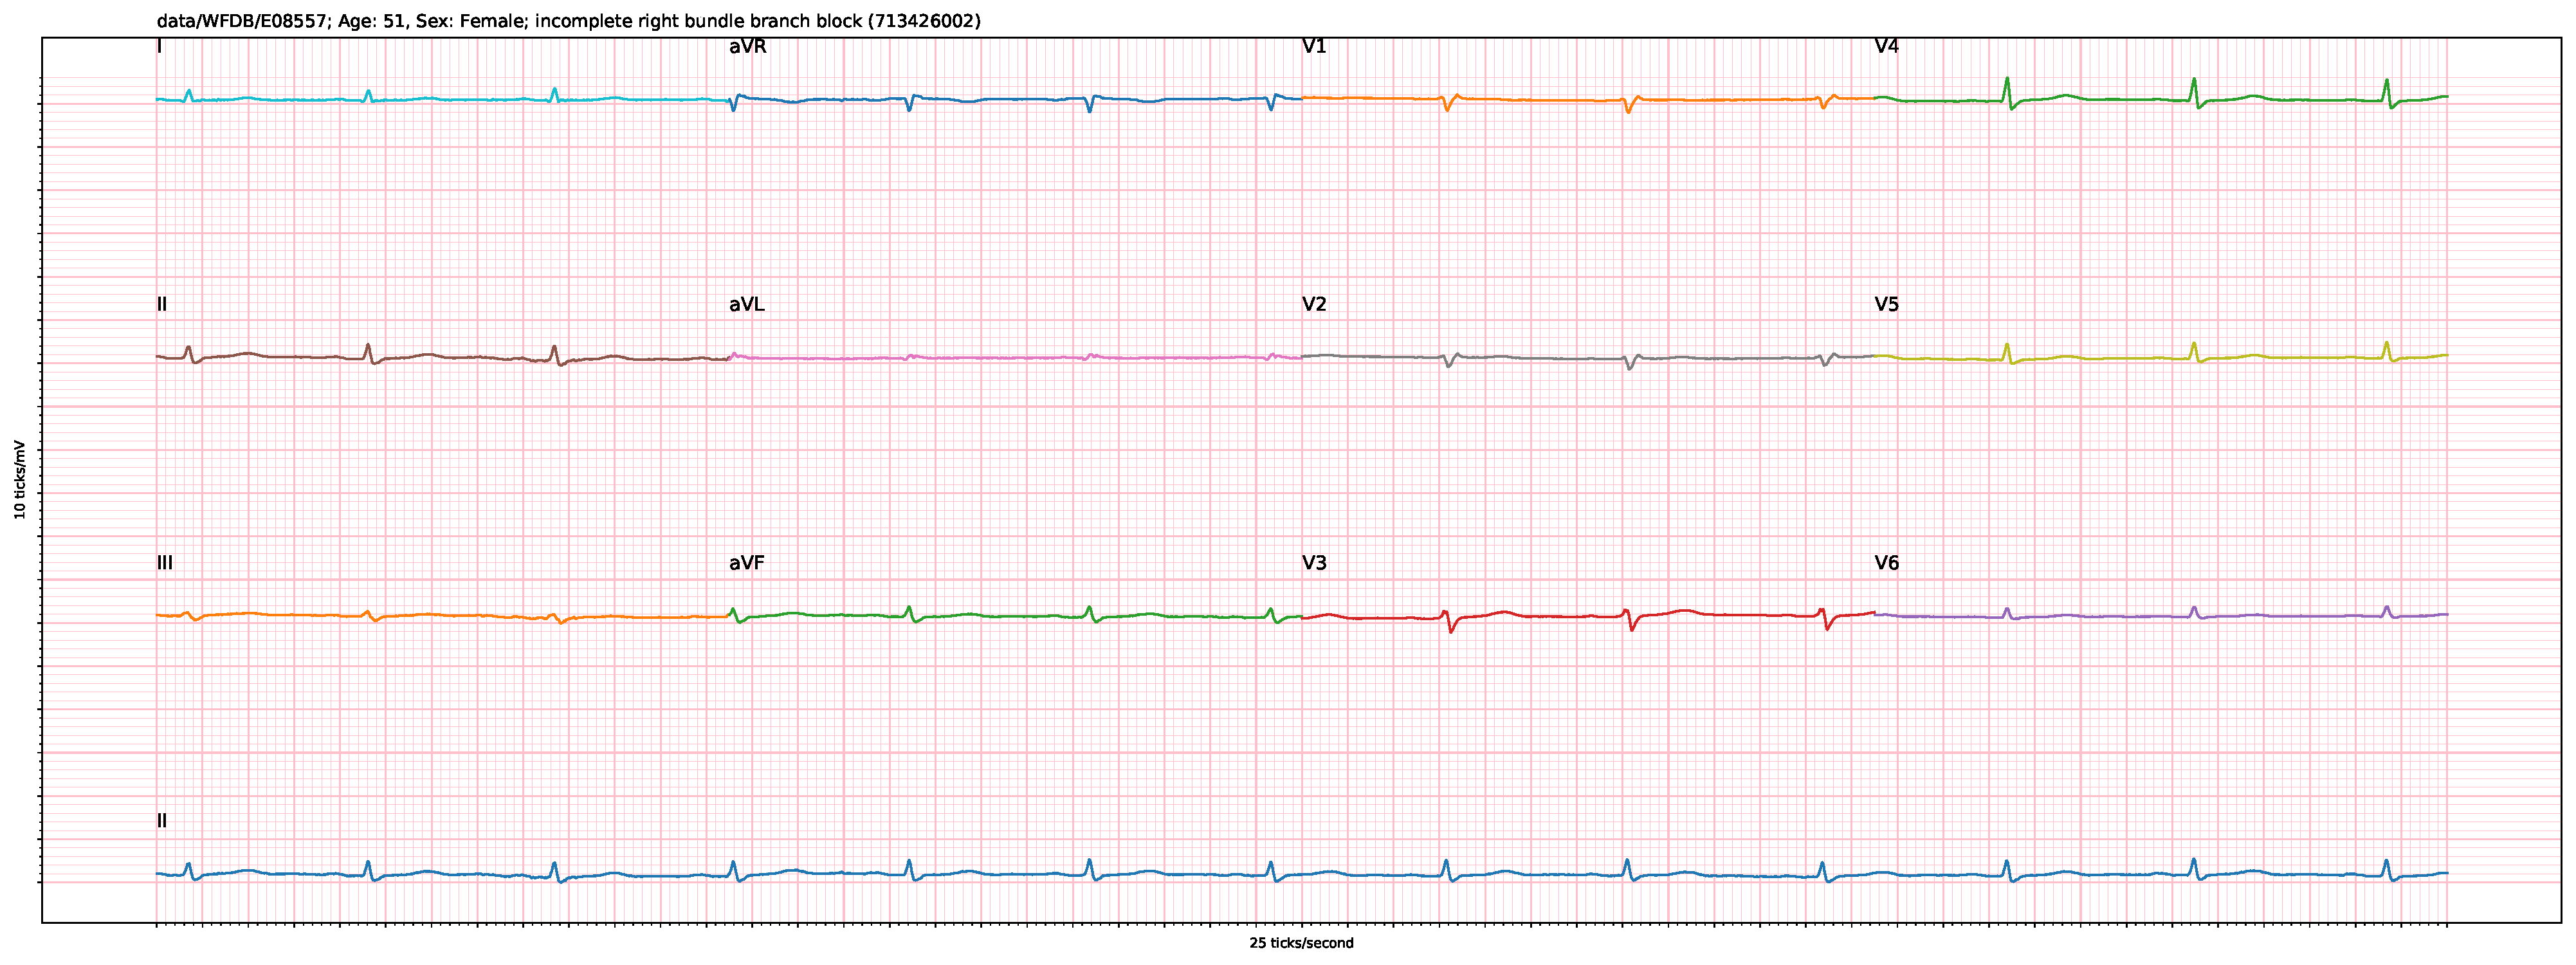
\includegraphics[width=14cm]{figure/IRBBB/full_28_18884.pdf}
        \caption{Instance of 12-lead \gls{ecg} with incomplete right bundle branch block. The QRS complex is within 100 to 120 ms (2.5-3 boxes) and contains an anterior skew on the right end of the QRS complex.}
        \label{fig:full_IRBBB}
    \end{figure} 
    \item[\gls{irbbb}] An incomplete right bundle branch block has the same terminal QRS features as \gls{crbbb} but has a QRS duration of 100 to 120 ms~\cite{ecg-utah-lesson}, as shown in the example record at Figure~\ref{fig:full_IRBBB}.
    \begin{figure}
        \centering
        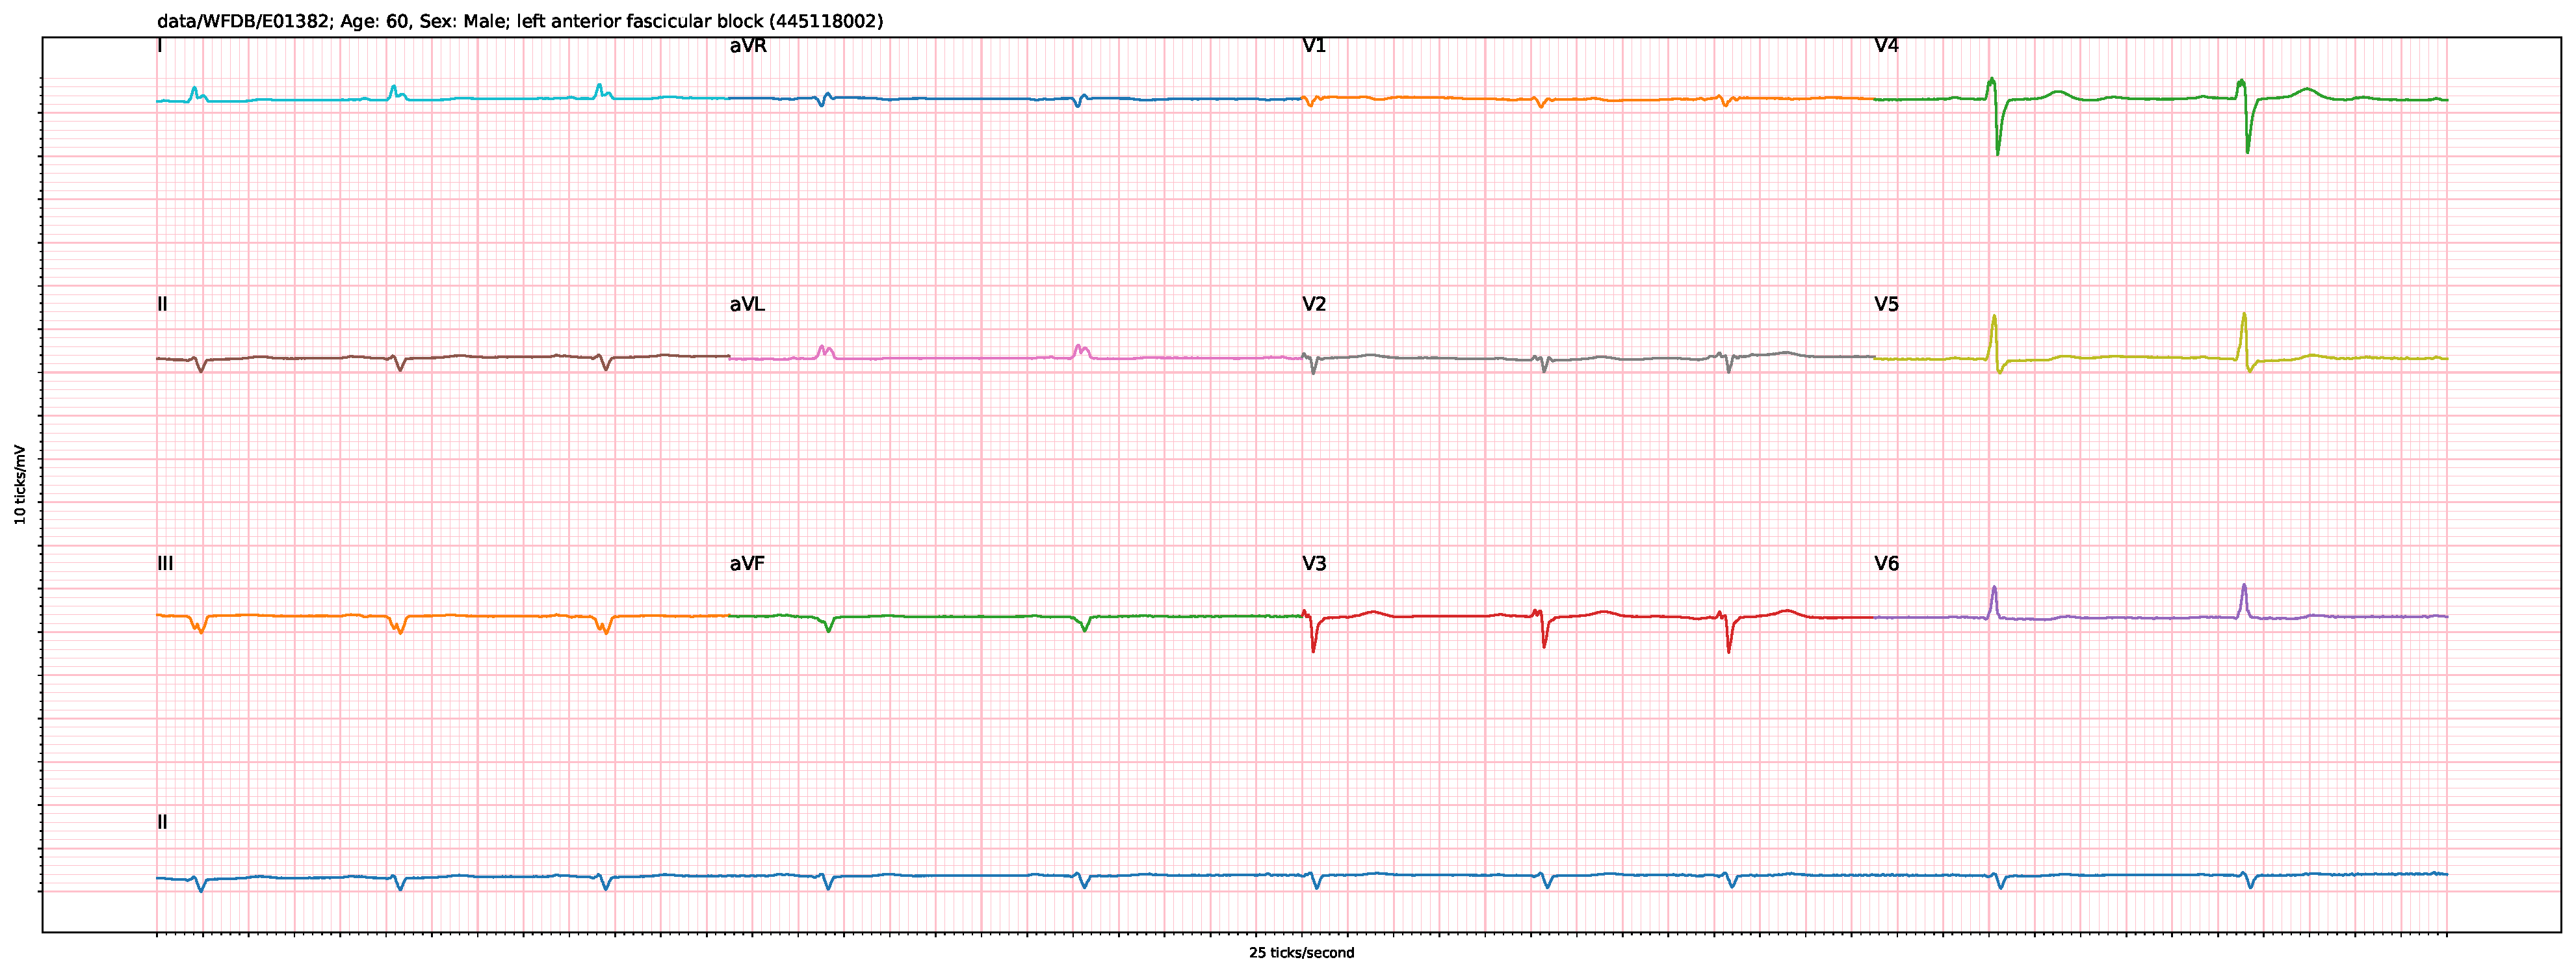
\includegraphics[width=14cm]{figure/LAnFB/full_3_11709.pdf}
        \caption{Instance of 12-lead \gls{ecg} with left anterior fascicular block. Lead I is positive while leads II and III are negative, indicating left axis deviation. Leads I and aVL show qR complexes, with rS complexes appearing in leads II, III, an aVF.}
        \label{fig:full_LAnFB}
    \end{figure} 
    \item[\gls{lanfb}] This common intraventricular defect occurs when the anterior fascicle within the left bundle branch is blocked or otherwise unable to respond to action potential stimuli~\cite{ecg-utah-lesson}. The criteria includes: left axis deviation (within $-45\deg$ to $-90\deg$); small Q waves with large R waves (`qR complexes') in leads I and/or aVL; small R waves with deep S waves (`rS complexes') in leads II, III, and aVF; slightly prolonged QRS duration (80-110ms), usually a poor R progression in leads V1, V2, and V3 with deeper S waves in leads V5 and V6. See Figure~\ref{fig:full_LAnFB} for an example.
    \begin{figure}
        \centering
        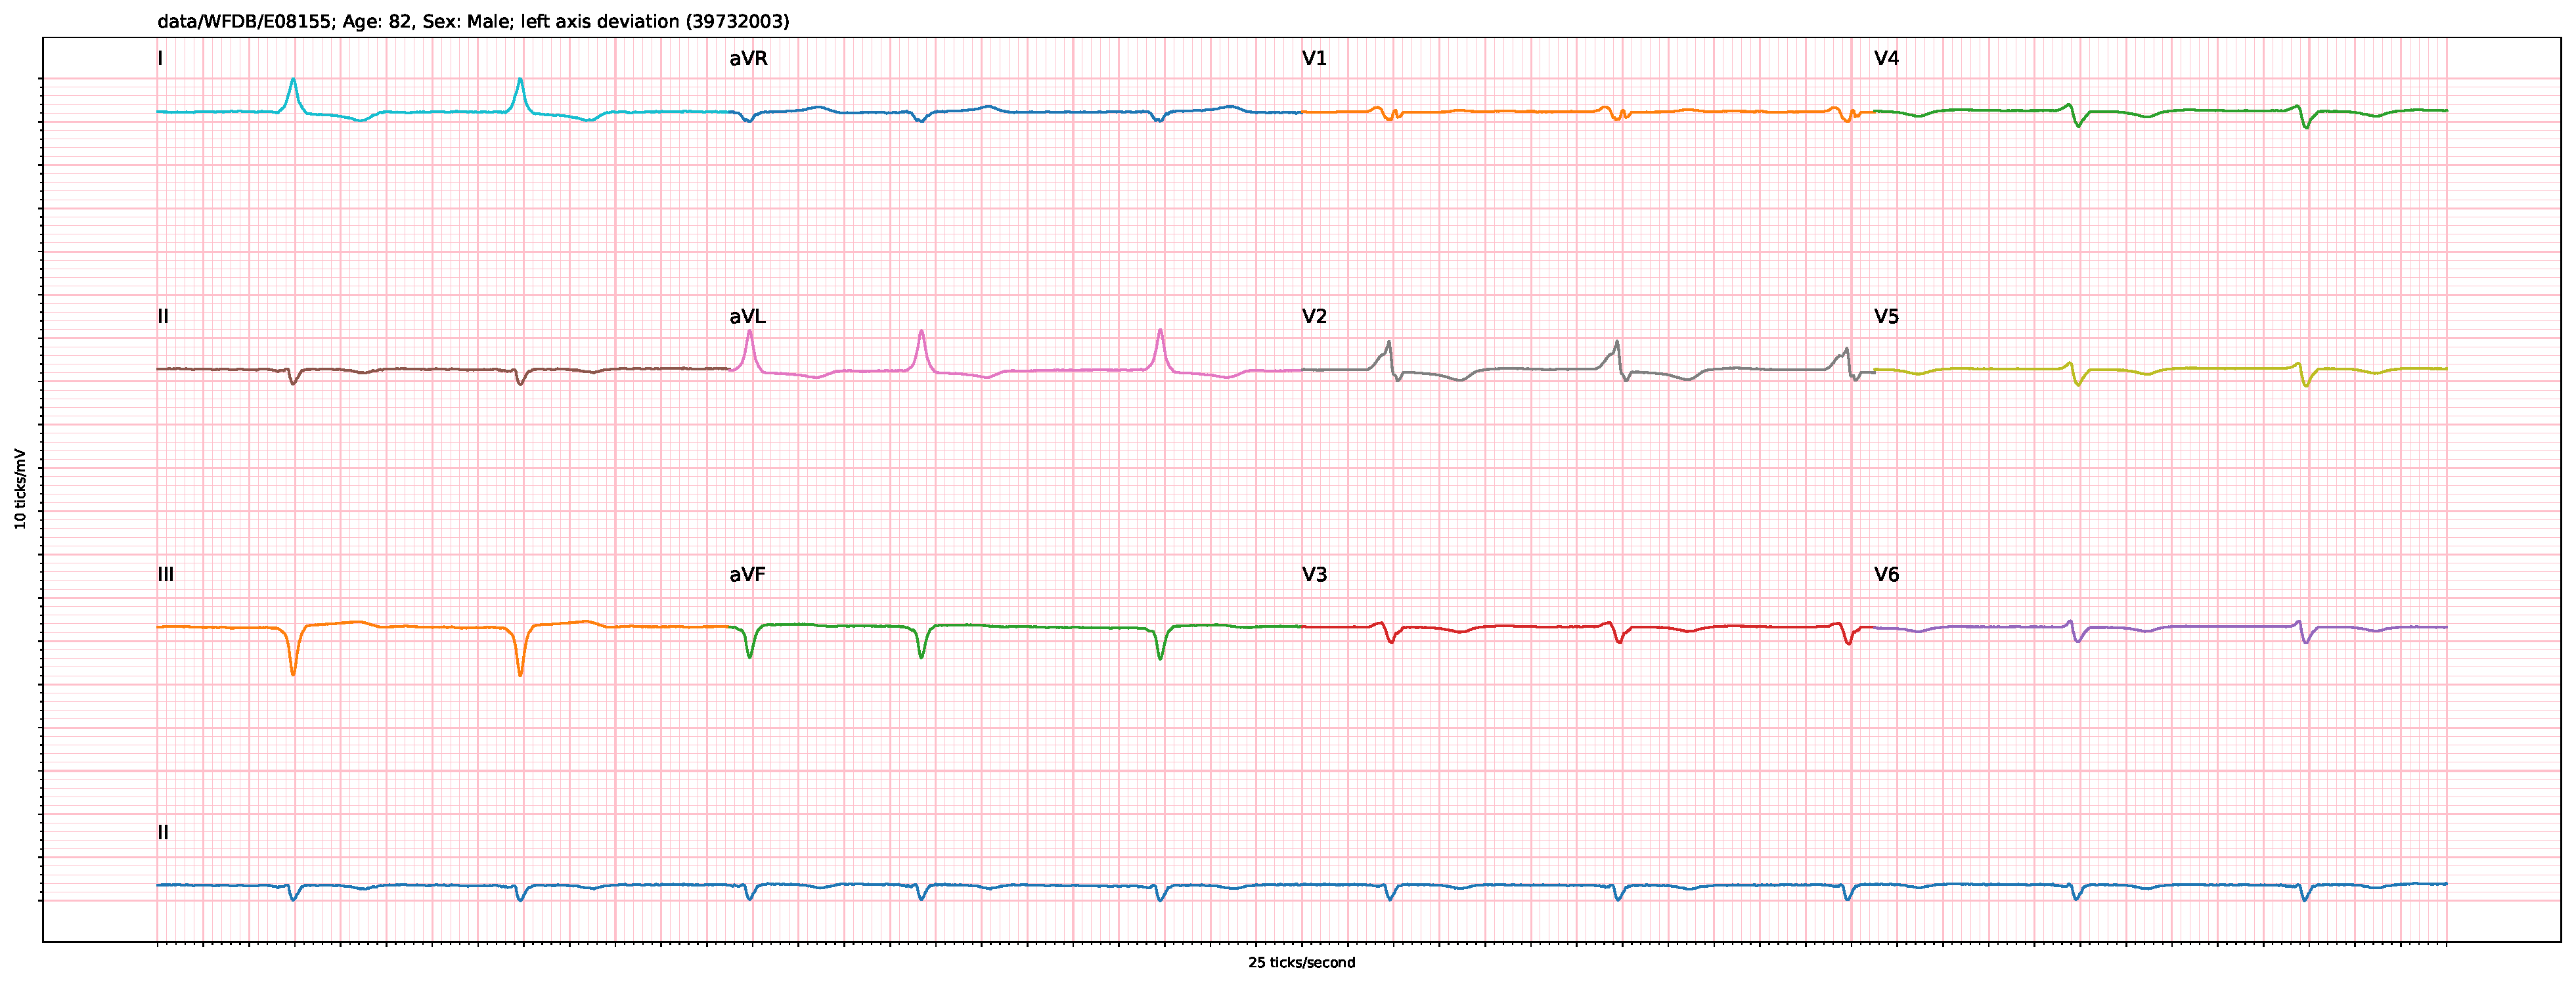
\includegraphics[width=14cm]{figure/LAD/full_69_18482.pdf}
        \caption{Instance of 12-lead \gls{ecg} with left axis deviation. Lead I is positive while leads II and III are negative.}
        \label{fig:full_LAD}
    \end{figure}

    \item[\gls{lad}] Diagnosed when the cardiac axis exists between $-30\deg$ and $-180\deg$.
    \item[\gls{lbbb}]
    \item[\gls{lqrsv}]
    \item[\gls{nsivcb}]
    \item[\gls{pr}]
    \item[\gls{pac}]
    \item[\gls{pvc}]
    \item[\gls{lpr}]
    \item[\gls{lqt}]
    \item[\gls{qab}]
    \item[\gls{rad}]
    \item[\gls{rbbb}]
    \item[\gls{sa}]
    \item[\gls{sb}]
    \item[\gls{snr}] The normal, healthy case for an \gls{ecg} record must have an upright P wave in leads I and II, with a QRS complex following each P wave~\cite{meek_introduction_2002}. In an adult, the resting heart rate should be between 60-99 beats per minute.
    \item[\gls{stach}]
    \item[\gls{svpb}]
    \item[\gls{tab}]
    \item[\gls{tinv}]
    \item[\gls{vpb}]
\end{description}

\subsection{Scoring Function}

% We plot an equation in figure \ref{fig:plot}.

% \begin{figure}
%     \centering
%     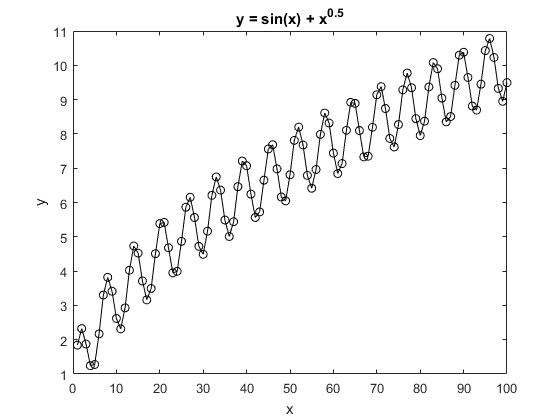
\includegraphics[keepaspectratio=true, width=0.9\textwidth]{\main/figure/plot}
%     \caption[A supporting figure] {A graph of $y = \sin(x) + \sqrt{x}$}
%     \label{fig:plot}
%     % Put the label *after* the caption, but inside the float
% \end{figure}

\end{document}